\vspace{-0.2cm}
\begin{flushright}
\emph{``Technique aussi brûlante que les derniers bilans du GIEC.''}\\
 Primero (ft. Romeo), in \textit{Deux deux}, 2022
\end{flushright}
\vspace{0.4cm}
%\medskip
%
%\begin{mybox}{Chapter overview}
%\begin{itemize}[left=0em]%[leftmargin=0cm,itemindent=.5cm,labelwidth=\itemindent,labelsep=0cm,align=left]
%\setlength\itemsep{-0.3em}
%\item Belgian energy system overview%Case studies: the Belgian energy systems during the transition (2015-2050).
%\end{itemize}
%\vspace{-0.3cm}
%
%\emph{This chapter is an improved and extended case study version of \citet{Limpens_belgian_2020}}.
%\end{mybox}
%
%\medskip

Assessing the robustness of a whole-energy system transition pathway calls a variety of methodological tools. First and foremost, such an extensive system needs to be represented, \ie modelled, to further be optimized. This model requires some characteristics to capture the peculiarities of this system such as the intermittency of \gls{VRES}, the coupling between the different energy and non-energy sectors and a pathway vision to pave the way from where we are to where we want to go.  Then, as looking into the future (\ie up to 2050 in this work) comes with its lot of uncertainties, these have to be assessed carefully in terms of characterisation and quantification. The former aims at defining the range over which parameters of the model vary. The latter allows assessing the impact that such uncertainties can have on the output of the model. Finally, meeting the environmental objectives while minimizing the cost of the system, accounting for this decision-making process, the uncertainties, and potential shocks/crisis, require therefore a framework to assess the relevance and the timing of the decisions throughout the transition. This work encompasses the optimisation of the policy,\ie set of actions to take along the transition with a specific methodology to assess its robustness. 

Detailing the different tools needed to answer the research questions, this chapter starts with the presentation of the whole-energy system optimization model, EnergyScope Pathway and its myopic formulation. Then, it focuses on the uncertainties, their characterisation as well as their quantification. Finally, an agent-based \acrfull{RL} approach is detailed to address the sequential decision-making process in the uncertain transition with limited vision in the future. The robustness of these policies is assessed via the use of the \gls{PCA}.

\section*{Contributions}
\label{sec:meth:contributions}
The main methodological contribution of this work is the implementation of the \gls{RL} approach to simulate and optimize the behaviour of an artificial agent interacting with its environment, \ie the the whole-energy system through its transition. Given the uncertainties and potential shocks of the future, this approach allows the agent to play the transition in a sequential, \ie myopic, way and optimize the choice and the timing of its actions. This optimization is done through trial and error where the agent repeats the transition with a new set of uncertainties. 

Then, to support this step-by-step transition with limited foresight in the future, we have extended the EnergyScope Pathway model \cite{limpens2021generating}. Originally developed to optimize the transition in one global optimisation up to 2050, \ie perfect foresight, part of this thesis consisted in making this model able to optimize the same transition but with sequential more limited time windows, \ie myopic approach. Besides its shorter computational time, this approach is more representative an actual decision process with limited foresight in the future \cite{babrowski2014reducing}.

The third principal methodological contribution is the use of \acrfull{PCA} to assess the robustness of a policy, \ie how much the optimal pathway is affected by the uncertainties. Given the uncertainties and the timespan of the transition, this approach allows highlighting the main \og directions'' of variation of the system design (\ie the installed capacities). After this step of identification, strategies and policies can be projected on these directions to see how robust they are to the overall transition uncertainties.

Finally, more minor methodological developments are part of this thesis. Following an approach similar to \citet{guevara2022modeling}, we have extended the ranges of uncertainty developed by \citet{Moret2017} to the pathway optimisation. After assessing the relevance of using \acrfull{PCE} on the optimisation of a whole-energy system \cite{limpens2020impact}, we have applied this uncertainty quantification method on the snapshot model subject to different emission-constraints \citet{rixhon2021role} as well as the pathway model. Eventually, starting from the initial investigation of \citet{goffauxpathway}, this work has converged to the most relevant formulation of the salvage value for the model EnergyScope. This aims at considering the residual value of assets that would still be in place after the end of the optimisation. It avoids penalising capital-intensive and long-lasting asset.In this formulation, the capacities that have been anticipatively decommissioned are removed from the total installed capacities. Therefore,  Therefore, this penalises decisions that would lead to investments that are later decommissioned before having reached the end of their lifetime.

\section*{Other authors' main contribution statement}
Novelty does not stand in the reinvention of the wheel.  This thesis, instead, finds its fundamentals in great tools previously developed by other authors. As developers of the building blocks of the main contributions of this thesis, three main authors are to be mentioned for having brought a significant part of the methodological work. Based on Stefano Moret's monthly whole-energy system model (\ie EnergyScope) \cite{moret2016strategic}, Gauthier Limpens has developed the hourly version of the snapshot model (\ie EnergyScope TD) \cite{limpens2019energyscope}, as well as the perfect foresight pathway model \cite{limpens2024pathway}, to which I personally contributed too. Diederik Coppitters has developed the RHEIA framework allowing to quantify the impact of uncertainties and carry out robust optimisation of energy systems \cite{coppittersthesis}. The current work used this framework for the first of these functionalities. Finally, Stefano Moret extensively assessed the uncertainty characterisation on the Swiss energy system \cite{Moret2017}. This thesis follows the same methodology, updating the uncertainty ranges for the pathway model.

\section{Whole-energy system transition model optimisation: EnergyScope Pathway}
\label{sec:meth:ES}

This work optimises the entire transition pathway from a known system in 2020 up to 2050 thanks to EnergyScope Pathway \cite{limpens2024pathway}. According to pathway models review (see Appendix \ref{app:ESPathway_choice}), EnergyScope Pathway can be categorised as an investment and operation optimisation model that assesses the whole-energy system, has a hourly time-resolution and is an open-source documented model. Moreover, it maintains a low computational cost (\ie around 15 minutes for a 30-year pathway with a hourly discretisation). From the perfect to the myopic foresight of the transition optimisation, this section presents only the main constraints of the former approach to further dig into more details about the latter. The reader is invited to refer to Appendix \ref{app:ESPathway_full_formulation} for more details about the formulation of the model and its extension from, EnergyScope TD, the a snapshot model, optimising a target future year with a greenfield approach \cite{geidl2006greenfield}. More extensive information about the formulation choices, for instance, can be found in \cite{limpens2024pathway} and the documentation \cite{readthedocs_pathway}.

\subsection{Perfect foresight: One global optimisation of the transition}
\label{subsec:meth:PF}

\begin{figure}[htbp!]
\centering
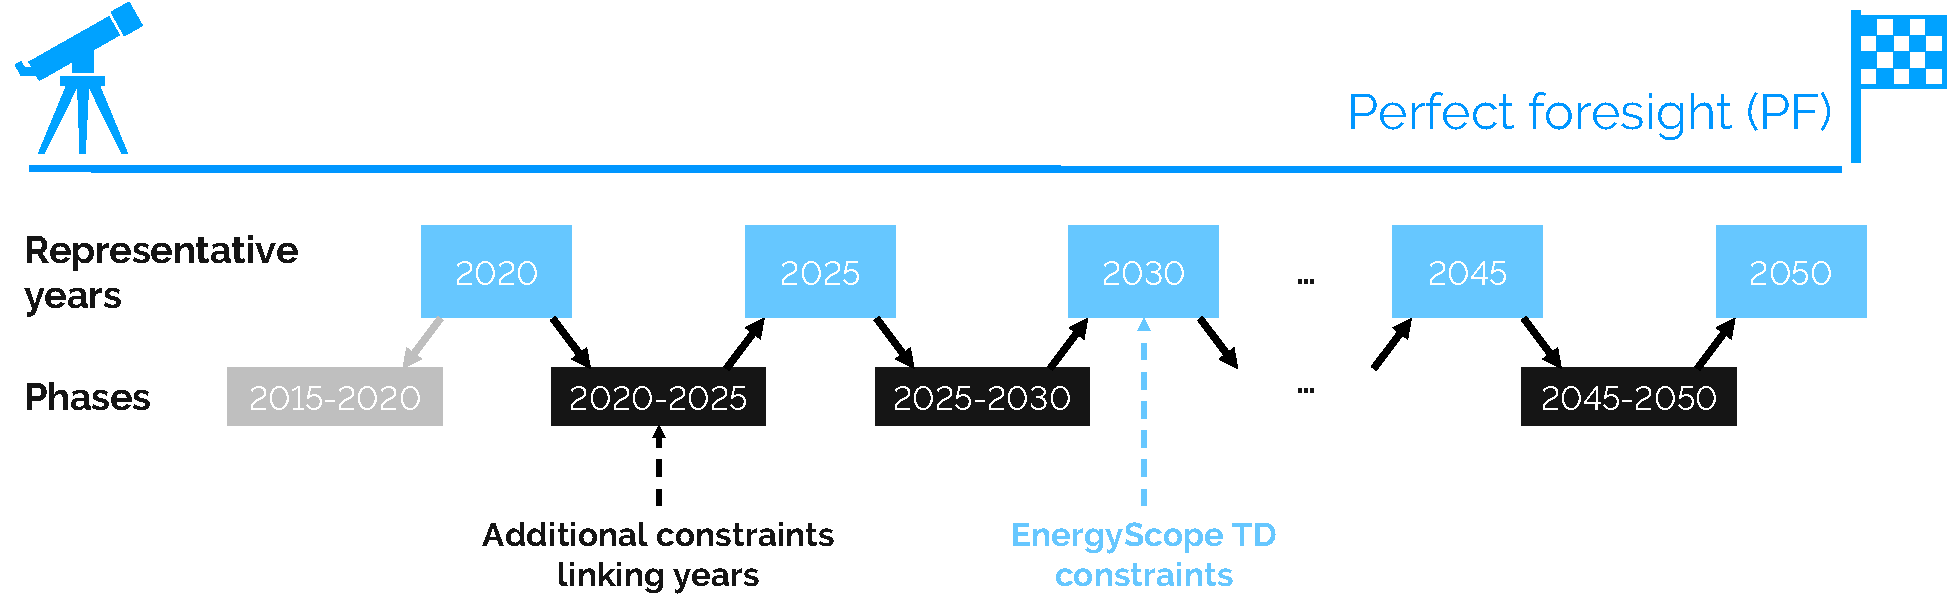
\includegraphics[width=\textwidth]{ES_Pathway.pdf}
\caption{Illustration of the pathway methodology based on an existing energy system model. The methodology spans from 2020 to 2050, with one representative year every five years. The model \acrfull{ESTD} is applied in 7 representative years (light blue boxes). The formulation includes additional constraints (black boxes) that link the years together. The pathway's initialisation assumes that all capacities installed in 2020 were built during the pseudo-phase of 2015-2020 (grey box). The overall problem is defined as the pathway model.}
\label{fig:meth_path_methodology_core}
\end{figure}

The whole-energy system model developed in this work originates from the perfect foresight (PF) formulation (\Cref{fig:meth_path_methodology_core}) of EnergyScope---the entire transition is computed in one optimisation, assuming a complete but uncertain knowledge of the different parameters until 2050 \cite{limpens2024pathway}. Each representative year is represented via the the variables and constraints of the snapshot model, EnergyScope TD \cite{limpens2019energyscope}. Then, to draw a consistent pathway between these years, additional constraints aim at linking them, \eg limiting the modal shifts within some energy sectors.

The objective function of the pathway model, \ie the total transition cost $\textbf{C\textsubscript{tot,trans}}$, is computed as the sum of the total \gls{CAPEX}, \textbf{C\textsubscript{tot,capex}}, and the \gls{OPEX}, \textbf{C\textsubscript{tot,opex}} (see Eq. \ref{eq:obj_func_v2}).

\begingroup
\vspace{-0.3cm}
\belowdisplayskip=2pt
\abovedisplayskip=2pt
\begin{flalign} 
% Objective function + investment 
\label{eq:obj_func_v2}%1
% adding 25pt space, otherwise flalign with two "&" would flush to the extreme 
\hspace{0pt} \min \text{  } & \textbf{C\textsubscript{tot,trans}} = \textbf{C\textsubscript{tot,capex}} + \textbf{C\textsubscript{tot,opex}}&%\\
\end{flalign}
\endgroup

%\label{eq:Capex_v2_app}
%& \textbf{C\textsubscript{tot,capex}} =
%\sum_{\mathclap{p \in \text{\emph{PHASE}}\cup \{2015\_2020\}}} 
%\textbf{C\textsubscript{inv,phase}}(p)
%-
%\sum_{\mathclap{i \in \emph{TECH}}} 
%\textbf{C\textsubscript{inv,return}}(i)\\
%  \label{eq:Copex_tot_v2_app}%5
%& \textbf{C\textsubscript{tot,opex}} =  \textbf{C\textsubscript{opex}}(2020)
%+ \emph{t\textsubscript{phase}}\cdot \tau\textsubscript{\emph{phase}}(p) \cdot \sum_{\mathclap{p \in \emph{PHASE}|y\textsubscript{start}\in \emph{P\_START}(p),y\textsubscript{stop}\in \emph{P\_STOP}(p)}} 
% \Big(\textbf{C\textsubscript{opex}}(y\textsubscript{start}) + \textbf{C\textsubscript{opex}}(y\textsubscript{stop}) \Big)/2&\\
%\label{eq:path_annu_factor_app}
%& \tau\textsubscript{\emph{phase}}(p) = 1/(1+\emph{i\textsubscript{rate}})^{\emph{diff\_2015\_year(p)}} &
%% GL_correction_v2 %% & \tau\textsubscript{\emph{phase}}(p) = 1/(1+\emph{i\textsubscript{rate}})^{\emph{diff\_2015\_year(p)}} &

The total \gls{CAPEX} is the difference between the total investments done during the transition, $\textbf{C\textsubscript{inv,phase}}$, and the residual value of the assets that would still be in place after the end of the transition, $\textbf{C\textsubscript{inv,return}}$ (see Eq.  \ref{eq:CAPEX_v2}).

\begingroup
\begin{flalign} 
\belowdisplayskip=2pt
\abovedisplayskip=2pt
\label{eq:CAPEX_v2}
\hspace{0pt}&\textbf{C\textsubscript{tot,capex}} =
\sum_{\mathclap{p \in \text{\emph{PHASE}}\cup \{2015\_2020\}}} 
\textbf{C\textsubscript{inv,phase}}(p)
- \sum_{\mathclap{j \in \emph{TECH}}} \textbf{C\textsubscript{inv,return}}(j),&
\end{flalign}
\endgroup

\noindent
where $\textbf{C\textsubscript{inv,phase}}$ is given as the sum over all the  newly installed technologies at the phase $p$, $\textbf{F\textsubscript{new}}(p)$, multiplied by the average investment costs, $\emph{c\textsubscript{inv}}$,  of the year starting and ending the corresponding phase, $\emph{y\textsubscript{start}}$ and $\emph{y\textsubscript{stop}}$ respectively (see Eq. \ref{eq:PhaseInv}).

\begingroup
\belowdisplayskip=2pt
\abovedisplayskip=2pt
\begin{flalign} 
\hspace{0pt} 
\label{eq:PhaseInv}%5
&\textbf{C\textsubscript{inv,phase}}(p) = \sum_{\mathclap{j \in \emph{TECH}}} \textbf{F\textsubscript{new}}(p,j)\cdot \tau\textsubscript{\emph{phase}}(p)\cdot \emph{c\textsubscript{inv}}(p,j)&\forall p \in \emph{PHASE},
\end{flalign}
\endgroup

\noindent where $\tau\textsubscript{\emph{phase}}$ is the annualised phase factor and $\emph{c\textsubscript{inv}}(p,j)$ is the arithmetic average of the investment cost of the technology $j$ at the beginning and the end of the phase, $\emph{c\textsubscript{inv}}(\emph{y\textsubscript{start}},j)$ and $\emph{c\textsubscript{inv}}(\emph{y\textsubscript{stop}},j)$. Similarly, the salvage value is computed in the proportion of the remaining years of life versus the initial lifetime of an installed capacity of a technology from which the anticipatively decommissioned part, $\textbf{F\textsubscript{decom}}$, is removed (see Eq. \ref{eq:salvage})

\begingroup
\belowdisplayskip=2pt
\abovedisplayskip=2pt
\begin{flalign} 
\label{eq:salvage}%5
&\textbf{C\textsubscript{inv,return}}(j) = \sum_{\mathclap{p \in \emph{PHASE}\cup \{2015\_2020\}}} 
\hspace{0.5cm}
 \tau_{phase}(p)\cdot \emph{c\textsubscript{inv}}(p,j) \cdot
&\notag\nonumber
\end{flalign}
\begin{flalign}
& 
\hspace{1.7cm}
\frac{remaining\_years(j,p)}{\emph{lifetime}(y\textsubscript{start},j)} \left( \textbf{F\textsubscript{new}}(p,j) - 
\sum_{\mathclap{p2 \in \emph{PHASE}}} 
\textbf{F\textsubscript{decom}}(p2,p,j)\right)&
\forall j \in \emph{TECH}
\end{flalign}
\endgroup

About the total \gls{OPEX} of the transition, $\textbf{C\textsubscript{tot,opex}}$, on top of the initial costs in 2020, we assume that the \gls{OPEX} of a phase is equal to the average operational costs, $ \textbf{C\textsubscript{opex}}$,  of $\emph{y\textsubscript{start}}$ and $\emph{y\textsubscript{stop}}$, multiplied by the duration of a phase $\emph{t\textsubscript{phase}}$ equal to 5 years in our case (see Eq. \ref{eq:Copex_tot_v2}).

\begingroup
\begin{flalign} 
  \label{eq:Copex_tot_v2}%5
&\textbf{C\textsubscript{tot,opex}} =  \textbf{C\textsubscript{opex}}(2020)
+ \emph{t\textsubscript{phase}}\cdot \tau\textsubscript{\emph{phase}}(p) \cdot \sum_{\mathclap{p \in \emph{PHASE}}} 
\textbf{C\textsubscript{opex}}(p),&
\end{flalign}
\endgroup

\noindent
where $\textbf{C\textsubscript{opex}}(p)$ is the arithmetic average of the operational cost at the beginning and the end of the phase $p$,  $\textbf{C\textsubscript{opex}}(y\textsubscript{start})$ and $\textbf{C\textsubscript{opex}}(y\textsubscript{stop})$. The operational cost of a year, $y$, $\textbf{C\textsubscript{opex}} (y)$, is the sum of the costs related to maintenance and operation of technologies, $ \textbf{C\textsubscript{maint}}$, and the consumption of resources, $\textbf{C\textsubscript{op}}$ (see Eq. \ref{eq:opex_yearly}).


\begingroup
\belowdisplayskip=2pt
\abovedisplayskip=2pt
\begin{flalign} 
\hspace{0pt} 
\label{eq:opex_yearly}
&\textbf{C\textsubscript{opex}} (y) = \sum_{\mathclap{j \in \emph{TECH}}} \textbf{C\textsubscript{maint}}(y,j) + \sum_{\mathclap{i \in \emph{RES}}} \textbf{C\textsubscript{op}}(y,i) & \forall y \in \text{\emph{YEARS}},
\end{flalign}
\endgroup

\noindent
where the costs related to each representative year are:

\begingroup
\belowdisplayskip=2pt
\abovedisplayskip=2pt
\begin{flalign} 
% Objective function + investment 
% adding 25pt space, otherwise flalign with two "&" would flush to the extreme left
\hspace{0pt} 
 \label{eq:c_maint}%4
 &\textbf{C\textsubscript{maint}}(y,j) = c_{\text{\emph{maint}}}(y,j) \textbf{F}(y,j) & \forall y \in \text{\emph{YEARS}}, \forall j \in \text{\emph{TECH}}\\ 
  \label{eq:c_op}%5
 &\textbf{C\textsubscript{op}}(y,i) = \sum_{\mathclap{t \in T }} c_{\text{\emph{op}}}(y,i) \textbf{F\textsubscript{t}}(y,i,t) t_{op} (t)  
 & \forall y \in \text{\emph{YEARS}}, \forall i \in \text{\emph{RES}},
 \end{flalign}
 \endgroup

\noindent where the variable $\textbf{F}$ represents the size of the installed capacities (for all technologies $j$) and the variable $\textbf{F\textsubscript{t}}$ is the hourly consumption of the resources; the parameter $c_{\text{\emph{maint}}}$ is the OPEX of the technologies, and the parameter $c_{\text{\emph{op}}}$ is the cost of purchasing resources. For the sake of simplicity, as done by \citet{limpens2024pathway}, the sum over the 8760 hours of the year is written as the sum over $t \in T $. 

he \ce{CO2}-budget for the transition, $\textbf{GWP\textsubscript{tot,trans}}$ is equal to the arithmetic average of the representative years at the beginning and the end of each phase (see Eq. \ref{eq:gwp_tot_transition}). Similarly to initial operational costs to account for the system in place in 2020 (see Eq. \ref{eq:Copex_tot_v2}), $ \textbf{GWP\textsubscript{tot}}(2020)$ accounts for the entire operational emissions in 2020, as the initial cumulative emissions of the transition. Then, as detailed in Section \ref{sec:cs:CO2-budget}, these cumulative emissions is constrained by a budget (see Eq. \ref{eq:limit_gwp_trans}).

\begingroup
\belowdisplayskip=2pt
\abovedisplayskip=2pt
\begin{flalign} 
\label{eq:gwp_tot_transition}
&\textbf{GWP\textsubscript{tot,trans}}= \textbf{GWP\textsubscript{tot}}(2020) + \emph{t\textsubscript{phase}}\sum_{\mathclap{p \in \emph{PHASE}}}\textbf{GWP\textsubscript{tot}}(p) &
\\
\label{eq:limit_gwp_trans}
& \textbf{GWP\textsubscript{tot,trans}} \leq \emph{gwp\textsubscript{lim,trans}},&
\end{flalign}
\endgroup

\noindent
where $\textbf{GWP\textsubscript{tot}}(p)$ is the arithmetic average of the yearly emissions at the beginning and the end of the phase $p$,  $\textbf{GWP\textsubscript{tot}}(y\textsubscript{start})$ and $\textbf{GWP\textsubscript{tot}}(y\textsubscript{stop})$. The computation of these yearly emissions are based on the \acrfull{GWP} of the resources:

\begingroup
\belowdisplayskip=2pt
\abovedisplayskip=2pt
\begin{flalign}
\hspace{0pt}
 \label{eq:GWP_tot}%8
 & \textbf{GWP\textsubscript{tot}}(y)  =    \sum_{\mathclap{i \in \text{\emph{RES}}}} \textbf{GWP\textsubscript{op}}(y,i) 
 & \forall y \in \text{\emph{YEARS}}\\
  \label{eq:GWP_op}%7
 & \textbf{GWP\textsubscript{op}}(y,i) = \sum_{\mathclap{t \in T }} gwp_{\text{\emph{op}}}(y,i) \textbf{F\textsubscript{t}}(y,i,t)  t_{op} (t) & \forall y \in \text{\emph{YEARS}}, \forall i \in \text{\emph{RES}},
\end{flalign}
\endgroup

\noindent
where $gwp_{\text{\emph{op}}}$ is the specific emissions (\ie in kt$_{\ce{CO2},\text{eq}}$/GWh) of each resource. Based on an approach developed by the Intergovernmental Panel on Climate Change (IPCC) \cite{stocker2014climate}, this work considers the indicator ``GWP100a - IPCC2013'' to compute the emissions related to the use of resources. This includes the emissions due to the extraction, the transportation and the combustion of the energy carrier. EnergyScope proposes to account for the embodied emissions of the technologies based on a \gls{LCA}. These stand for extraction of materials, refining, construction and end of life \cite{schnidrig2023integration}. However, this work is still in progress and the database is not yet complete. Consequently, it is not included in this work and not accounted for.

Besides this constraint on the emissions, the main constraint to link years with each other is the one dictating the installed capacities at the end of each year:

\begingroup
\belowdisplayskip=2pt
\abovedisplayskip=2pt
\begin{flalign} 
\label{eq:F_newBuilt}%5
&\textbf{F}(y\textsubscript{stop},j) = \textbf{F}(y\textsubscript{start},j)
 + \textbf{F\textsubscript{new}}(p,j)
 - \textbf{F\textsubscript{old}}(p,j)
 - \sum_{\mathclap{p2 \in \text{\emph{PHASE}} \cup \{2015\_2020\}}} \textbf{F\textsubscript{decom}}(p,p2,j)& \notag \nonumber 
 \end{flalign}
\begin{flalign} 
 &&  \forall p \in \text{\emph{PHASE}}, \emph{y\textsubscript{stop}} \in \emph{Y\_STOP}(p), \emph{y\textsubscript{start}} \in \emph{Y\_START}(p), j \in \text{\emph{TECH}}
 \end{flalign}
\endgroup

\noindent
where the variables $\textbf{F\textsubscript{old}}$ and $\textbf{F\textsubscript{decom}}$ are the capacities respectively having reached the end of their lifetime and prematurely decommissioned. Moreover, to account for the society inertia and to prevent unrealistically fast modal share change, constraints limit this change for the sectors of the low-temperature, the passenger mobility and freight mobility demands. The interested reader will find more information about the formulation choices related to it in the work of \citet{limpens2024pathway}. 

\subsection{Myopic: Sequential optimisation of the transition with limited foresight}
\label{subsec:meth:MY}

One of the main methodological contributions of this work regarding the development of the whole-energy system model consists in giving it the possibility to optimise the transition pathway in a myopic approach.After introducing the general concept of it, this section details more the additions brought to the model in terms of implementation.\\

\myparagraph{General concept of the myopic optimisation}\\

\begin{figure}[htbp!]
\centering
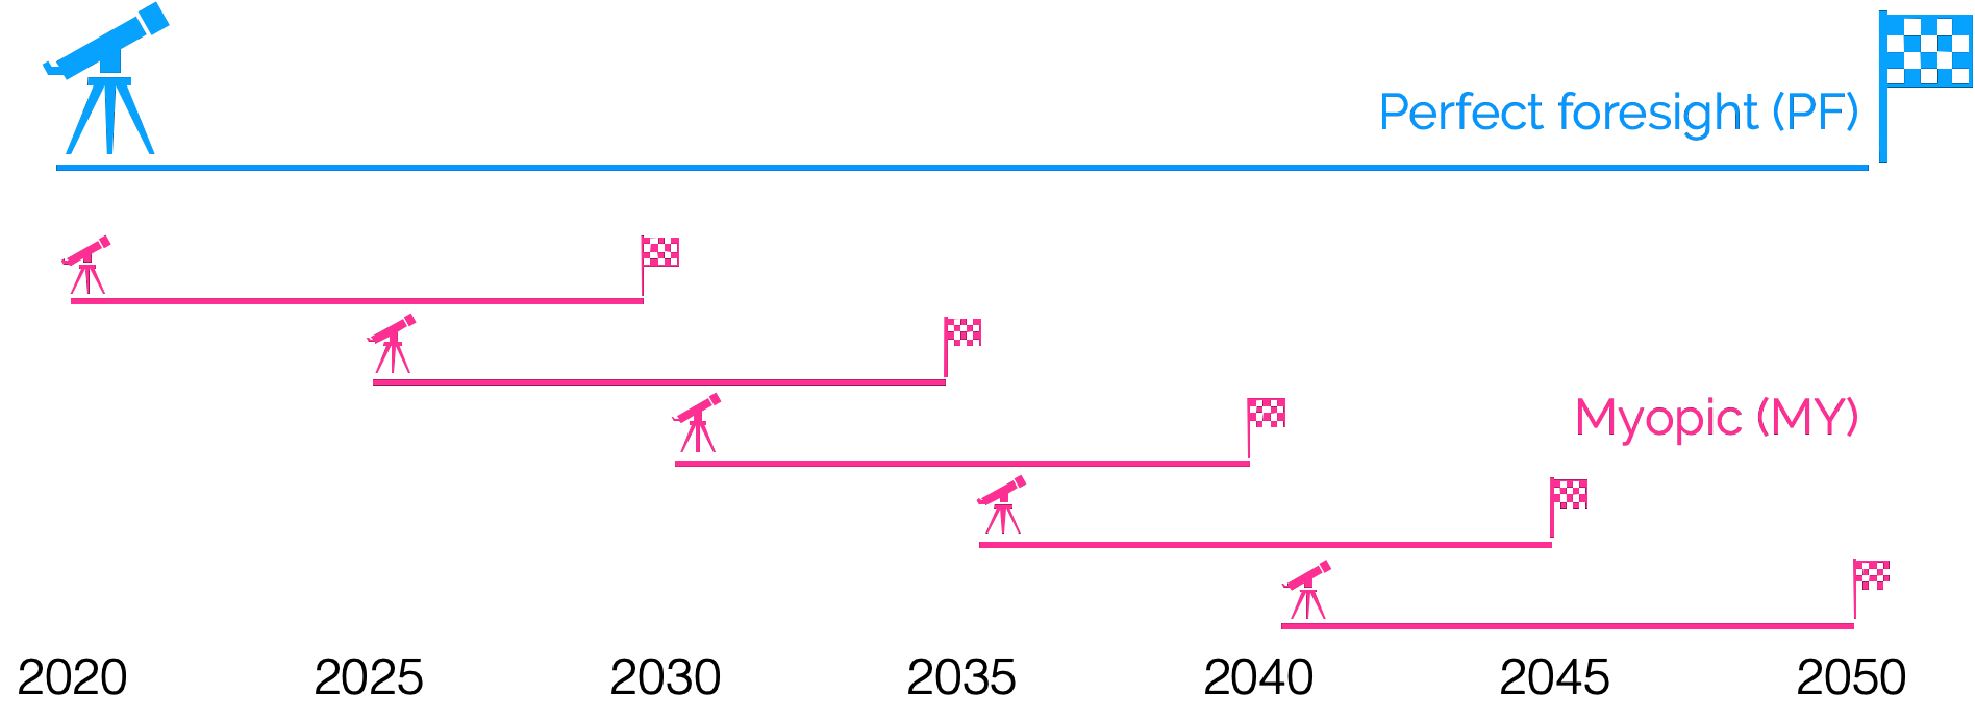
\includegraphics[width=\textwidth]{MY_schematic.pdf}
\caption{The myopic approach (in pink) uses several instances of the pathway model (illustrated in Figure \ref{fig:meth_path_methodology}). In this example, the pathway instance has a time horizon of 10 years ($N\textsubscript{year,opti}=10$) with a 5 year-overlap ($N\textsubscript{year,overlap}=5$). As a comparison the Perfect foresight (in blue) has a time horizon of 30 years.}
\label{fig:my_schematic}
\end{figure}

\noindent
Compared to the perfect foresight, the myopic approach (Figure \ref{fig:my_schematic}) has two main advantages: shorter computational time and more realistic representation of the short-sightedness of decision-makers. For this reason, several studies are based on this approach \citep{babrowski2014reducing,poncelet2016myopic,nerini2017myopic,heuberger2018impact}. \citet{babrowski2014reducing} analysed the benefit of the myopic approach to reduce the computational time. \citet{poncelet2016myopic} uses this approach to analyse the expansion planning of the power sector beyond 2050 to assess the realism of the decision making process brought up by the myopic implementation. \citet{nerini2017myopic} analysed the impact of the horizon windows and overlapping time.  Overall these studies decided to choose the myopic approach to analyse the speed of change compared to a perfect foresight approach.
 % rajout du Réalisme 
Moreover, the myopic approach allows a sequential optimisation process that opens the doors to decision-making/policy-learning methodologies, like assessing shock events. This approach is used by \citet{heuberger2018impact} who assessed the speed of integration of technologies due to these events. 
In their analysis of the overcapacity in European power systems, \citet{moret2020overcapacity} emphasised that such a ``possibility of \textit{recourse}" is very appropriate to address uncertainty gradually unfolding over time. Consequently, the development of the myopic approach with an overlap between two successive time windows has been implemented. This sequential optimisation framework also represents the foundations of the further implementation of the agent-based reinforcement learning framework (see Section \ref{sec:meth:RL}).

As illustrated in Figure \ref{fig:my_schematic_2}, after optimising, in design and operation, one time window (\eg from 2020 to 2030), the intermediate system design (\ie the installed capacities) is set as initial conditions for the start of the next time window (\eg from 2025 to 2035) as well as the historical investment decisions (\ie $\textbf{F\textsubscript{new}}$, $\textbf{F\textsubscript{old}}$ and $\textbf{F\textsubscript{decom}}$). Consequently, the solution obtained at the end of the first time window (\eg 2030) as well as potential investment decisions between the start of the second time window and this end-year are discarded. In other words, they are not taken into account for the optimisation of the second time window since the new final year is further into the future. This process goes on until the stated end of the transition (\ie 2050, in this case).

\begin{figure}[htbp!]
\centering
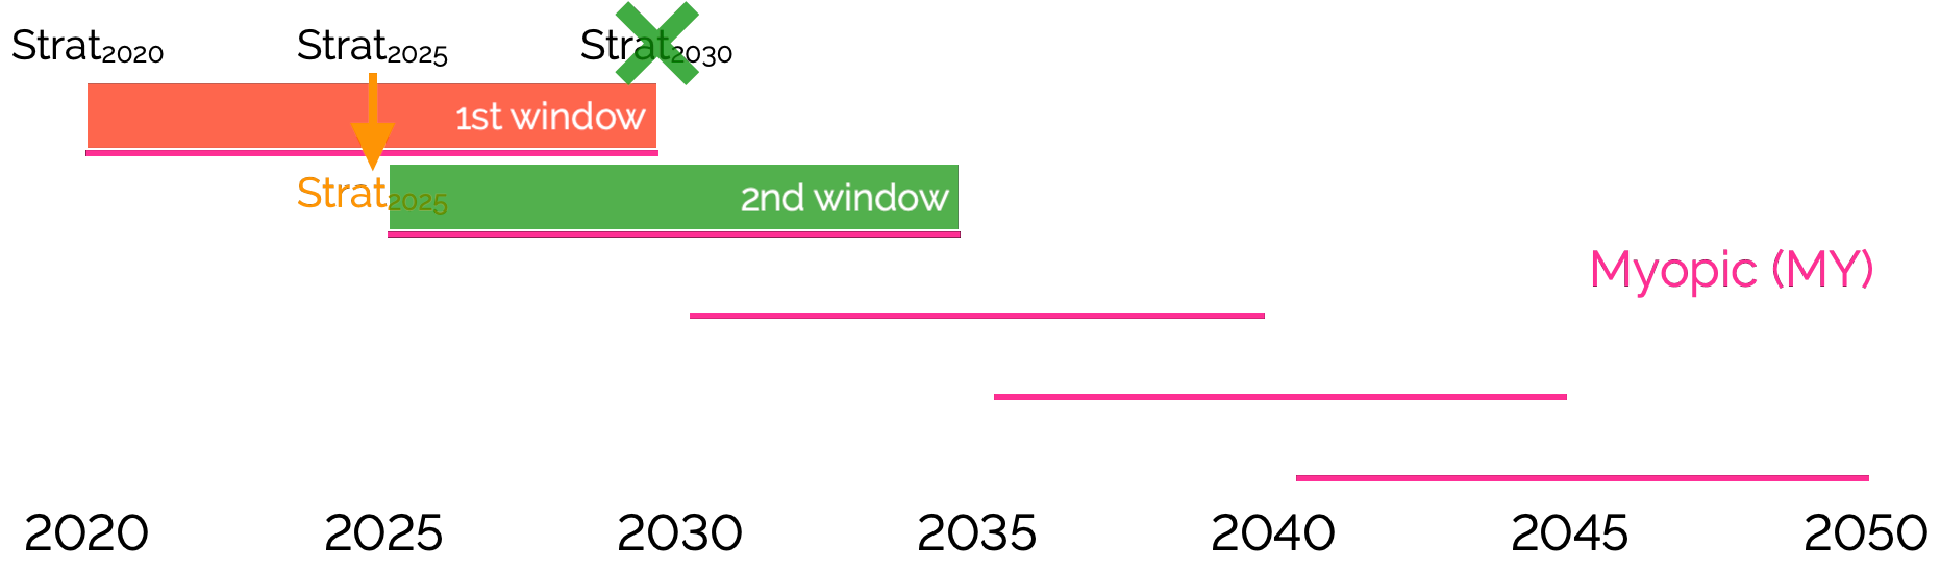
\includegraphics[width=\textwidth]{MY_schematic_2.pdf}
\caption{Sequential optimisation of the transition pathway in the myopic approach: (i) first time-window optimisation, (ii) set-up of the initial conditions of the second time-window, (iii) second time-window optimisation discarding intermediate results}
\label{fig:my_schematic_2}
\end{figure}

\myparagraph{Additional sets, parameters and variables}\\

\noindent
The major add-on from the original EnergyScope Pathway model \cite{limpens2021generating} to the myopic version developed in this thesis, is the possibility to carry out the optimisation on a limited time window, of which the duration is defined by $N\textsubscript{year,opti}$. Moreover, there is also the possibility of having an overlap between two consecutive time windows. The timespan of this overlap is defined by the parameter $N\textsubscript{year,overlap}$. The philosophy followed behind the development of the myopic approach was to add another layer on top of the perfect foresight model in order to make it more modular. For this reason, the already existing constraints are marginally adapted. This way, the newly developed model can easily be used to perform a perfect foresight optimisation by setting the time window to $N\textsubscript{year,opti}=$30 years (\ie between 2020 and 2050) and the overlap between the time windows to $N\textsubscript{year,overlap}=$0.  Consequently, as it is fundamental to define, on the one hand, the actual time window on which the system is optimised, and on the other hand, the history, \ie what has already been optimised earlier in the transition, four new sets are implemented: $\text{YEARS}\textsubscript{WND}$, $\text{YEARS}\textsubscript{UP TO}$, $\text{PHASE}\textsubscript{WND}$ and $\text{PHASE}\textsubscript{UP TO}$ (see Table \ref{tab:path_my_sets}).

\begin{table}[htbp]
\caption[New SETs for myopic pathway formulation.]{New SETs for myopic pathway formulation.} 
\label{tab:path_my_sets}
%\begin{minipage}{\textwidth}
\centering
%\resizebox{\textwidth}{!}{
\begin{tabular}{l c l}
\toprule
\textbf{Set}      & \textbf{Index}	 &	\textbf{Description}\\
\midrule
$\text{YEARS}\textsubscript{WND}$ 	&	$y\in$Y	& 	\pbox{20cm}{\vspace{1mm} Representative years of the \\ time window to optimize}\\
$\text{YEARS}\textsubscript{UP TO}$ &	$y\in$Y	& 	\pbox{20cm}{\vspace{1mm} Representative years including the \\ years already optimised, \ie the history}\\
$\text{PHASE}\textsubscript{WND}$ &  $\emph{p}\in$P & 	\pbox{20cm}{\vspace{1mm} Phases of the time window to optimize}\\
$\text{PHASE}\textsubscript{UP TO}$ &  $\emph{p}\in$P & 	\pbox{20cm}{\vspace{1mm} Phases including the phases \\ already optimised, \ie the history}\\
\bottomrule
\end{tabular}%}
%\end{minipage}
\end{table}

$\text{YEARS}\textsubscript{WND}$ and $\text{PHASE}\textsubscript{WND}$ substitute $\text{YEARS}$ and $\text{PHASE}$ in the constraints defined in the pathway model in Section \ref{subsec:meth:PF}. These two sets aim at setting the optimization to a more limited time window. Progressing through the transition, $\text{YEARS}\textsubscript{UP TO}$ and $\text{PHASE}\textsubscript{UP TO}$ allow keeping track of the history of the investments (\eg technologies installation, decommissioning or retirement), the consumption of resources, the cumulative amount of emissions, etc.

On top of these four specific sets, some artefacts were also necessary to avoid computational rounding errors. For instance, the first year of a time window is the result of the optimisation of the previous one. Therefore, optimising again this first year could lead to rounding errors preventing from the optimization to converge. For this reason,  the set $\text{YEAR}\textsubscript{ONE}$ accounts for the first representative year of the time window to optimize that is excluded from $\text{YEARS}\textsubscript{WND}$ to avoid these errors. This remark stays valid for any time window except the first one of the transition where the year 2020 is optimized even though its technological strategy is set according to the actual system presented in Appendix \ref{app:bel_2020}. Finally, as the end of time windows changes for each of them, the parameter $remaining\_years$ has to be updated accordingly to keep a meaningful definition of $\textbf{C\textsubscript{inv,return}}$ in Eq. \ref{eq:salvage}.\\

\myparagraph{Myopic pathway implementation}\\

\noindent
Starting this work in 2017, AMPL Optimization Inc. has developed a Python \gls{API} called amplpy \cite{amplpy}. In a nutshell, this API allows the pre/post-processing of an ampl optimisation problem by accessing its features (\eg constraints,parameters, variables, objective function) from within Python. Using this\gls{API}, this updated version of the model interacts with the AMPL problem representing the optimization of the whole-energy system transition pathway as represented in Figure \ref{fig:MY_process_code}. 


\begin{figure}[htbp!]
\centering
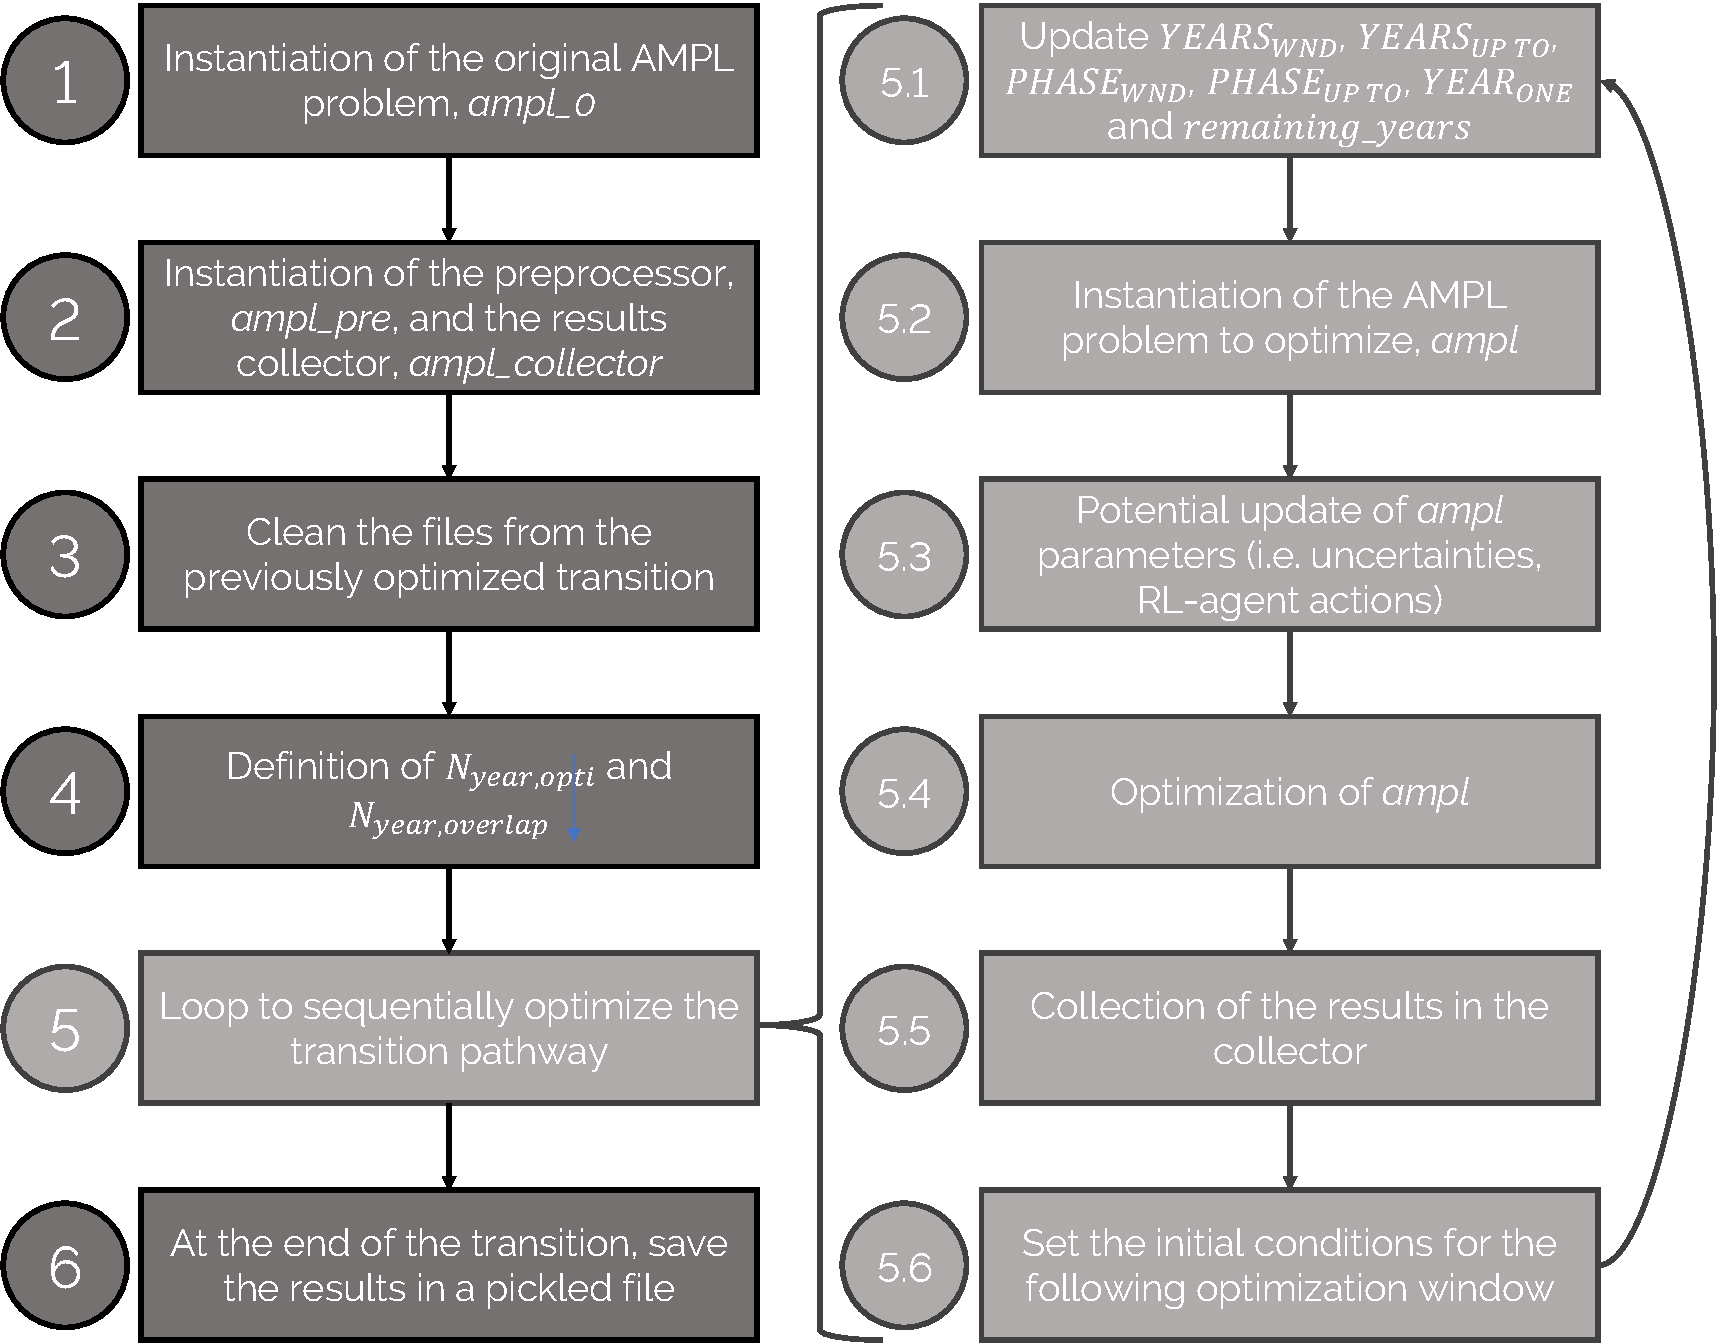
\includegraphics[width=10cm]{MY_process_code.pdf}
\caption{Schematic of the iterative optimization of the whole-energy system transition pathway.}
\label{fig:MY_process_code}
\end{figure}

\myparagraph{Impact of myopic formulation on the system}\\

\noindent
In line with the work of \citet{babrowski2014reducing}, the computational time is reduced drastically (\ie by 55\%). On top of this, we observed that the resulting design, \ie the technological mix, remains similar.  Given the continuous change of the input parameters over the considered time frame, the perfect foresight and myopic approaches results are very similar, like in \cite{krey2006vergleich}: less than 1\% cost difference over the transition, similar system designs by 2050 and slight shifts in time in terms of adoption of technologies. 

The main difference lies in the myopic transition itself and especially in the earlier deployment of PVs and offshore wind turbines. These induce the reinforcement of the grid that is a capital-intensive and long-lifetime asset. This is mostly due to impact of the salvage value, Eq. \ref{eq:salvage}, in the objective function. Since this is now the transition cost over a more limited time window (\ie 10 years rather than 30 years), a bigger salvage value, deduced from the total investments, leads to a temporary better optimum at early stages of the transition. A more detailed comparison between the myopic and perfect foresight approaches is available in Appendix \ref{app:my_vs_pf}.

\section{Uncertainty quantification}
\label{sec:meth:UQ}
In their systematic review, \citet{yue2018review} highlighted that a wide majority of studies addressing the optimisation of energy systems (\ie 75\% out of the 134 reviewed studies) were not investigating the impact of uncertainties. However, disregarding these impacts can have drastic consequences on the system design. For instance, historical low \gls{NG} prices have led to overcapacity of \gls{CCGT} in Europe \cite{moret2020overcapacity}. This is why accounting for uncertainty in \gls{ESOMs} is crucial \cite{mavromatidis2018uncertainty}, especially when it comes to optimise several decades in an inherently uncertain future \cite{peace2008insights}.

This section aims at briefly presenting the methods followed to first characterise these uncertainties, then to quantify their impact on different outputs of interest of the model (\eg amount of molecules imported from abroad, the installed capacity of \gls{SMR} or the total transition cost) and finally, the screening and selection of the parameters to analyse.

\subsection{Uncertainty characterisation}
\label{subsec:uncert_charac}
Characterising precisely the uncertainty---ideally with their respective probability density functions (PDFs)---of the thousands of parameters in the model is daunting if not impossible because of lack of data \cite{marnay2006addressing}. Therefore, we used a workaround developed by \citet{Moret2017} that defines relative ranges of variation for different groups of parameters. These ranges have been adapted for the Belgian energy system and the pathway formulation. Moreover, some ranges have been added to account for new parameters coming from the pathway formulation described in Section \ref{sec:meth:ES} like the society inertia. Like other works \cite{li2019renewables,coppitters2021robust} and given the scarcity of information, the uncertain parameters are assumed to be independent and uniformly distributed between their respective lower and upper bounds. Alternatives like PERT or Gaussian distributions could also have been considered \cite{coppittersthesis}.

%\Cref{tab:UC_short} gives the uncertainty ranges of some key parameters. A particular attention is to pay to the potential installation of \gls{SMR}, at the bottom of \Cref{tab:UC_short}. As detailed in \Cref{sec:cs:technologies}, the commercial availability of such a technology is uncertain but would not be before 2040. Consequently, for \gls{SMR}, the parameter $f_{\mathrm{max,SMR}}$ influences the maximum capacity to install to translate somehow the readiness of this technology. As SMRs are foreseen, if installed, to be around the same locations (\ie Tihange and Doel) as the conventional nuclear power plants and using the same area in kW/ha, the same 6\,GW are assumed to be the maximum capacity for SMRs. If it is (i) smaller than 0.6, there is no possibility to install \gls{SMR} during the transition; (ii) between 0.6 and 0.8, these 6~GW can be installed only in 2050; (iii) between 0.8 and 0.9, these can be installed from 2045 onward and; (iv) higher than 0.9, the prescribed maximum capacity can be installed from 2040 onward. Based on the local sensitivity analysis carried out by \citet{PATHS2050}, the current work also considers a [-40\%; +44\%] range on the CAPEX of SMR, on top of the uncertainty about the availability. Finally, the the cost of purchasing renewable electrofuels presents a wide range, [-64.3\%; +179.8\%], like the other imported commodities.

%The exhaustive list of the parameters accounted in this work is presented in Appendix \ref{app:UC_full}.

%\begin{table}[htbp!]
%\caption{Illustration of the uncertainty characterisation for different parameters for the year 2025. $^{(a)}$ Per \cite{Moret2017PhDThesis}, \og I: investment-type, II: operation-type (constant uncertainty over time), III: operation-type (uncertainty increasing over time)\fg. $^{(b)}$ The nominal value of each parameter is 0, meaning no variation compared to the nominal values of the impacted parameter in the model. $^{(c)}$ This range has been inferred from the local sensitivity analysis performed by \citet{PATHS2050}.}
%\label{tab:UC_short}
%\centering
%\resizebox{\textwidth}{!}{
%\begin{tabular}{l l l c c c}
%\toprule
%\multirow{2}{*}{\textbf{Category}} & \multirow{2}{*}{\textbf{Parameter}} & \multirow{2}{*}{\textbf{Meaning}} & \multirow{2}{*}{\textbf{Type}$^{(a)}$}  & \multicolumn{2}{c}{\textbf{Relative variation$^{(b)}$}}\\
%    & & & &	 min 	&	 max \\ 	
%\midrule		
%\multirow{2}{*}{\textbf{Cost of purchasing}} & $c_{\mathrm{op,fossil}}$ & Purchase fossil fuels & II & -64.3\% & 179.8\% \\
%& $c_{\mathrm{op,electrofuels}}$ & Purchase electrofuels & II & -64.3\% & 179.8\% \\
%\midrule
%\multirow{5}{*}{\textbf{Investment cost}} &$c_{\mathrm{inv,car}}$ & CAPEX car  & I & -21.6\% & 25.0\% \\
%& $c_{\mathrm{inv,e\_prop}}$ & CAPEX electric motor & I & -39.6\% & 39.6\% \\
%& $c_{\mathrm{inv,fc\_prop}}$ & CAPEX fuel cell engine & I & -39.6\% & 39.6\% \\
%& $c_{\mathrm{inv,PV}}$ & CAPEX PV & I & -39.6\% & 39.6\% \\
%& $c_{\mathrm{inv,nuclear\_SMR}}$ & CAPEX \gls{SMR}$^{(c)}$ & I & -40.0\% & 44.0\% \\
%\midrule
%\multirow{1}{*}{\textbf{Consumption}} &$\eta_{\mathrm{e\_prop}}$ & Consumption electric vehicles & I & -28.7\% & 28.7\% \\
%\midrule
%\multirow{2}{*}{\textbf{Potential installed capacity}} &$f_{\mathrm{max,PV}}$ & Max capacity PV & I & -24.1\% & 24.1\% \\
%& $f_{\mathrm{max,windon}}$ & Max capacity onshore wind & I & -24.1\% & 24.1\% \\
%\midrule
%\multirow{2}{*}{\textbf{Hourly load factor}} & $c_{\mathrm{p,t,PV}}$ & Hourly load factor PV & II & -22.1\% & 22.1\% \\
%& $c_{\mathrm{p,t,winds}}$ & Hourly load factor wind turbines & II & -22.1\% & 22.1\% \\
%\midrule
%\multirow{2}{*}{\textbf{Resource availability}} & $avail_{\mathrm{elec}}$ & Available electricity import & I & -32.1\% & 32.1\% \\
%& $avail_{\mathrm{biomass}}$ & Available local biomass & I & -32.1\% & 32.1\% \\
%\midrule
%
%\multirow{2}{*}{\textbf{End-use demand}} & $pass\_EUD$ & Passenger mobility EUD & III & -7.5\% & 7.5\% \\
%& $industry\_EUD$ & Industry EUD & III & -20.5\% & 16.0\% \\
%\midrule
%
%\multirow{4}{*}{\textbf{Miscellaneous}} &$i_{\mathrm{rate}}$  & Interest rate & I & -46.2\% & 46.2\% \\
%& $\Delta_{\mathrm{change,freight}}$ & Modal share change freight mobility & - & -30\% & 30\% \\
%& $\Delta_{\mathrm{change,pass}}$ & Modal share change passenger mobility & - & -30\% & 30\% \\
%& $f_{\mathrm{max,SMR}}$ & Potential capacity \gls{SMR} & - & 0 & 1 \\
%
%\bottomrule							
%
%\end{tabular}}
%\end{table}

Following the methodology defined by \citet{Moret2017}, uncertainties of types I (investment-type) and II (operation-type, constant uncertainty over time) keep the same range width for the whole transition. In other words, unlike type III parameters, this width is not expanding (nor narrowing) for the different representative years of the transition. However, parameters with an uncertainty increasing over time, type III, (\ie end-use demands, in this case) will have a wider and wider range over the transition (see Figure \ref{fig:ranges_transition}). In this work, a +50\% linear increase has been set between the width of the range of such parameters in 2025 and the same ranges in 2050. This choice leads to an industrial \gls{EUD} that could be, in 2050, -30.8\% compared to its nominal value. This potential drop compared to the reference is in line with the work of \citet{My2050}. In their work, the total energy demand in the industry sector in 2050 could be between -19\% to -50\% of the reference value, depending on the scenario. In \Cref{fig:ranges_transition}, this means that for type III uncertainties only, $R_{2050}^+$ is 50\% bigger than $R_{2025}^+$ and $R_{2050}^-$ is 50\% smaller than $R_{2025}^-$. For uncertainties of types I and II, the relative variation versus the nominal value remain the same over the transition. Inspired by \citet{guevara2022modeling}, the values of the uncertain parameters are set at a fixed relative position from the nominal values for each sampled transition---the values do not zigzag from 2025 to 2050 within the bounds (\Cref{fig:ranges_transition}).

\begin{figure}[htbp!]
\centering
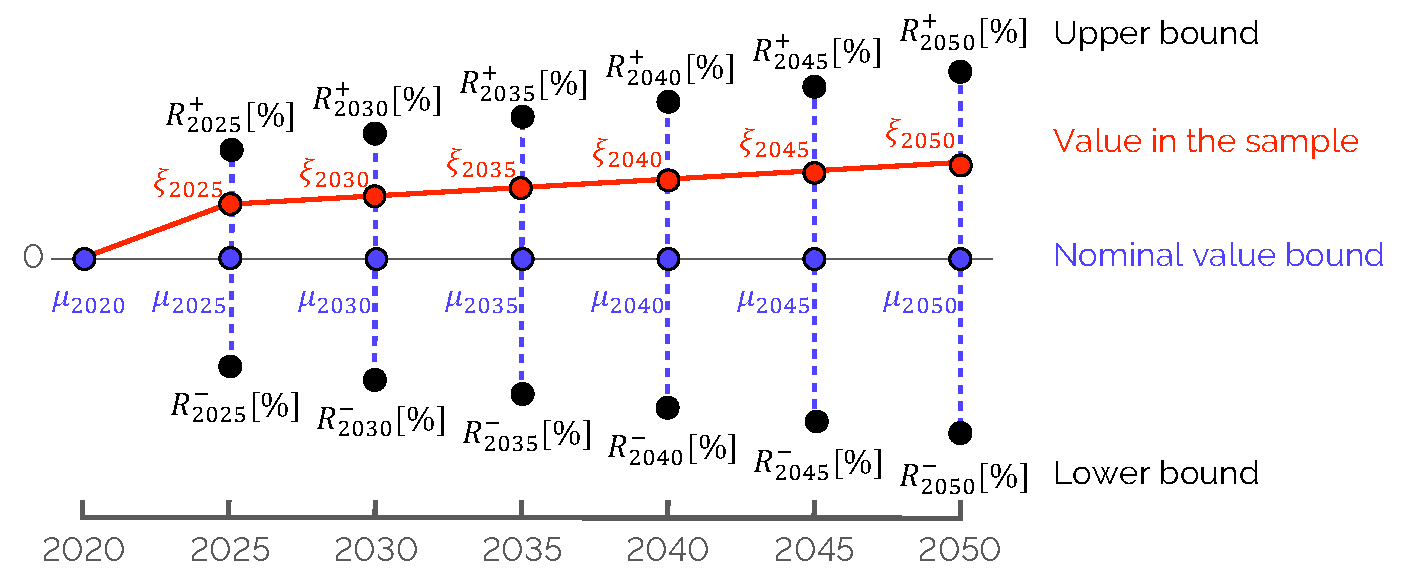
\includegraphics[width=0.7\textwidth]{ranges_transition.pdf}
\caption{Expansion of the width of uncertainty range for type III parameters. $\mu_{2020}$, $\mu_{2025}$, ...,  $\mu_{2050}$ are the nominal values equal to 0 as the uncertain parameters represent a relative increase/decrease of actual parameters of the model. $R^+$ and $R^-$ are respectively the upper and lower bounds of the range and $\xi_{2025}$, $\xi_{2030}$, ...,  $\xi_{2050}$ are the values taken by one parameter for a specific sample of the \gls{GSA} for each of the representative years of the transition, always starting from the nominal value in 2020, $\mu_{2020}$. The graph has been adapted from \cite{guevara2022modeling}.}
\label{fig:ranges_transition}
\end{figure}

Finally, the model accounts for thousands of parameters. The computational burden to consider all of them separately would be completely overwhelming ($\sim 10^7$ model runs\footnote{As detailed in Section \ref{subsec:pce}, the number of runs required for the \gls{GSA} is proportional to the factorial of the number of uncertain parameters. As second order \gls{PCE} is the minimum to ensure accuracy of the surrogate model, considering thousands of independent uncertain parameters would lead to millions of runs, if no more.}). Similarly to other works \cite{Moret2017,limpens2020impact}, the model parameters that would follow the same uncertainty have been grouped to one single uncertain parameter. On top of mitigating the computational burden, this aims at grouping parameters that are closely linked with each other. For instance, the uncertainty on the cost of purchasing renewable electrofuels, $c_{\mathrm{op,electrofuels}}$, identically affects the cost of e-hydrogen, e-methane, e-ammonia and e-methanol. Indeed, besides their respective specificities, each of these fuels will be similarly affected by the variation of cost of electricity or the electrolyser, that drive the majority of their cost of purchasing \cite{h2coalition}. Similarly, the uncertainties impacting the industrial demand, $industry\_\emph{EUD}$, alters equally the industrial high- and low-temperature and electricity demands as well as the non-energy demand.

\subsection{Polynomial Chaos Expansion}
\label{subsec:pce}

To avoid the avoid the computational burden of well-known method like Monte-Carlo analysis \cite{yue2018review}, we used \gls{PCE} to carry out a \gls{GSA}. \gls{PCE} is an approach for surrogate-assisted \gls{UQ} that propagates uncertainties in input parameters through the system model. This allowed us to assess statistical moments on the quantity of interest and determine Sobol' indices~\cite{coppitters2020robust}. To construct a PCE of the EnergyScope Pathway model, we employed the open-source Python framework RHEIA~\cite{coppitters2022rheia,readthedocs_rheia}. Where the first part of this section is dedicated to the mathematical definition of this approach, the second details its choice and summarises the comparison made with another approach (\ie Morris method) in a previous work \cite{limpens2020impact}.\\

\myparagraph{Definition}\\

\noindent
The PCE model ($\hat{M}$) is a representation of the relationship between the input parameters and the output variable of interest (\ie the value of the objective function, see Eq. \ref{eq:obj_func_v2}) in the EnergyScope Pathway model ($M$). This representation is constructed as a truncated series of multivariate orthonormal polynomials $\bm{\Psi}$, weighted by coefficients $u$:

\begin{equation}
\hat{M} \left( \bm{\xi} \right) = \sum_{\bm{\alpha} \in \mathcal{A}^{d,p}} u_{\bm{\alpha}} \bm{\Psi}_{\bm{\alpha}} \left( \bm{\xi} \right) \approx M \left( \bm{\xi} \right), 
\end{equation}

\noindent where the vector $\bm{\xi} = (\xi_1,\xi_2, \dots \xi_d)$ comprises the independent random input parameters (\autoref{app:UC_full}), $d$ corresponds to the number of input distributions and $\bm{\alpha}$ is a multi-index, \ie a vector of non-negative indices of length $d$, where each index corresponds to the degree of each univariate polynomial that forms the basis of the multivariate polynomial $\bm{\Psi_{\bm{\alpha}}}$. The coefficients ($u_0, u_1, \dots, u_{P+1}$) are quantified using a regression method applied to orthonormal polynomials~\cite{Sudret2014}. As uniform distributions are considered, the Legendre polynomials are adopted, as they are the associated family of polynomials that are orthogonal with respect to standard uniform distributions~\cite{Sudret2014}.

A truncation scheme is implemented to restrict the number of multivariate polynomials in the series. This is done based on two factors: a specified limiting polynomial order ($p$) and the number of uncertain parameters ($d$) involved. The multivariate polynomial order $|\bm{\alpha}|$ is the summation of the orders for each univariate polynomial in the multivariate polynomials space. Thus, only the multi-indices corresponding to an order that is less than or equal to the specified limiting order are retained and stored in the truncated series denoted as $\mathcal{A}^{d,p}$:

\begin{equation}
\mathcal{A}^{d,p} = \left \{ \bm{\alpha} \in \mathbb{N}^d : |\bm{\alpha}| \leq p \right \}. 
\end{equation}

The number of multi-indices satisfying this condition is as the cardinality of $\mathcal{A}$, \ie the number of its elements:
\begin{equation}
\mathrm{card} \left( \mathcal{A}^{d,p} \right) = {p + d \choose p} = \dfrac{\left( d + p \right) !}{d! p!} = P + 1.
\label{eq:pce:nterms}
\end{equation}

To ensure a well-posed least-square minimisation, it is recommended to have a number of training samples at least twice the number of coefficients~\cite{Sudret2014}. Therefore, $2 \left( P+1 \right)$ samples are evaluated in the system model, and the model response for each quantity of interest is recorded. To generate the training samples, the quasi-random Sobol' sampling technique is employed~\cite{bratley2003implementing}. As a low-discrepancy sequence, this technique exhibits the main advantage to investigate efficiently and (almost) uniformly the hypercube of uncertainties, unlike uniformly distributed random numbers.

The process of defining the polynomial degree includes incrementally increasing it until a desired level of accuracy is achieved~\cite{coppitters2022rheia}. Starting with $p=1$, a PCE is constructed and the \gls{LOO} error is evaluated. If the \gls{LOO} error is below a specified threshold ($\sim 1\%$), the corresponding polynomial order is considered sufficient for generating an accurate PCE. However, if the error exceeds the threshold, the order is increased, and additional samples are generated following the rule of Eq.\,(\ref{eq:pce:nterms}).

For the specific study of this work, a polynomial order of 2 is necessary (with 1260 training samples as per Eq.\,(\ref{eq:pce:nterms})) to achieve a \gls{LOO} error below \SI{1}{\%} for the total transition cost.

Lastly, the statistical moments can be analytically derived from the PCE coefficients, eliminating the need for further model evaluations. The mean $\mu$ and standard deviation $\sigma$ are obtained as follows:
\begin{align}
\mu &= u_0,\\
\sigma^2 &= \sum_{i \neq 0 } u_{i}^2 .
\label{eq:pce:statmom}
\end{align}

Furthermore, the Sobol' indices can also be determined analytically. The total-order Sobol' indices ($S_i^{T}$) assess the overall influence of a stochastic input parameter on the performance indicator, encompassing all possible interactions:

\begin{equation}
S_i^{T} = \sum_{\bm{\alpha} \in A_i^T}^{} u_{\bm{\alpha}}^2/\sum_{i=1}^P u_i^2 ~~~~~~ A_i^T = \{\bm{\alpha} \in A | \alpha_i > 0\}.
\end{equation}

Here, $A$ denotes the collection of all PCE coefficients, and $\alpha_i$ corresponds to the coefficient associated with the uncertain parameter $i$.\\

\myparagraph{Comparison with a proven method}\\

\noindent
Besides being an in-house used method, an early step of this thesis consisted in assessing \gls{PCE} with similar approach used in the literature \cite{limpens2020impact}. 

After characterising the uncertainty ranges, \citet{Moret2017} quantified the impact of these uncertainties on the snapshot model of EnergyScope,  \ie ranking them, using the Morris method \cite{morris_factorial_1991}.  This method, as a statistical analysis, relies on individually randomized one-factor-at-a-time designs. Given the $d$ model parameters $\vec{\xi}=(\xi_1,\xi_2,...,\xi_d)$, the first step of the method consists in generating independent random samples of $\vec{\xi}$ in a standardised and discretised $p$-level \textit{region of experimentation}, $\omega$. In this \textit{region of experimentation}, each $\xi_i$, varying in the interval $[\xi_{i,min},~\xi_{i,max}]$, can take a random discrete value as follows :
\begin{equation}
  \xi_{i}=\xi_{i,min}+j\cdot\frac{1}{p-1}\left(\xi_{i,max}-\xi_{i,min}\right)~~\text{with }j\in\{0,1,...,p-1\}
\end{equation}

Then, given these random one-factor-at-a-time samples, Morris method defines, for a given set of $\vec{\xi}$, the elementary effect of the $i$th parameter ($EE_i$) as :
\begin{equation}
  EE_{i}=\frac{M(\xi_1,\xi_2,...,\xi_i+\Delta,...,\xi_d)-M(\vec{\xi})}{\Delta},
\end{equation}

\noindent where $M$ is the objective function, $\vec{\xi}\in\omega$, except $\xi_i\leq1-\Delta$ and $\Delta$ is a set multiple of $1/(p-1)\left(\xi_{i,max}-\xi_{i,min}\right)$. As in other studies \cite{Sin2009,Moret2017,Moret2017PhDThesis}, we consider $p$ as even and $\Delta=p/[2(p-1)]\left(\xi_{i,max}-\xi_{i,min}\right)$.\\

Finally, in order to evaluate the importance of the $i$th parameter over an output, Morris method relies on $F_i$, the distribution of $r$ elementary effects. Computing the mean, $\mu_{i}=\mu(F_{i})$, and the standard deviation, $\sigma_{i}=\sigma(F_{i})$, of the $F_{i}$ distribution, allows ranking the parameters based on their influence on the concerned output. Usually, in Morris method, $p$ and $r$ respectively get values as follows : $p\in \{4,6,8\}$ and $r\in [15;100]$ depending on, $d$, the number of uncertain parameters. The higher this number is,  the higher shall be, simultaneously, $p$ and $r$. In the following comparative analysis, we set $p$ and $r$ to their maximum values, respectively $8$ and $100$ in order to get the most reliable parameters ranking.\\

Beyond the original Morris method, we used the standardized elementary effects, $SEE_{i}$, formulation \cite{Sin2009}, given by
\begin{equation}
    SEE_{i}=EE_{i}\cdot\frac{\sigma(\xi_i)}{\sigma(M)}.
\end{equation}
Among other things, the $SEE$ allows comparing the influence of different inputs on the same output or compare the influence of a same parameter on different outputs, even if these parameters or outputs are significantly different in terms of variation range or average amplitude. Moreover, this standardized analysis does not require any additional model evaluations.\\
Therefore, in the following results, we rather use
\begin{equation}
\mu^*_{i}=\mu(\vert SF_{i}\vert)
\label{eq:mu*}
\end{equation}

to rank parameters among each other. In (\ref{eq:mu*}), $SF_{i}$ is the distribution formed by the $r$ standardized elementary effects, as done in \citet{Moret2017PhDThesis}.

In \cite{limpens2020impact}, we have assessed the \gls{PCE} approach, comparing the Top-14 most impacting parameters obtained from this approach with the one provided by the improved Morris method based on $\mu^*_{i}$. Even if the output of each method does not have the same physical meaning, both methods can rank the parameters by their impact on the total annual  cost  of  the  energy  system. Both rankings were very similar which validates the use of \gls{PCE} in the rest of this work.


\subsection{Preliminary screening and selection}
\label{subsec:screening}

After the initial phase of grouping (Section \ref{subsec:uncert_charac}), a preliminary screening was necessary to identify the key parameters to account for in this \gls{GSA}. \citet{rixhon2021role} performed a similar sensitivity analysis on the 2050 Belgian whole-energy system under different \ce{CO2}-limits using the snapshot model, \ie EnergyScope TD \cite{limpens2019energyscope}. Screening the results of this work, we have discarded some parameters with negligible impact\footnote{Per \citet{Turati2017}, parameters are considered as ``negligible'' if their Sobol' index is below the threshold $=1/d$, $d$ being the total number of uncertain parameters} (\eg CAPEX of electrolysers or variation of the freight demand), selected a subset of parameters and added others that were intrinsic to the pathway formulation, \eg modal share changes, or related to the integration of \gls{SMR}, $f_{\mathrm{max,SMR}}$. The exhaustive list of these 34 parameters is presented in Appendix \ref{app:UC_full}.


\section{Agent-based reinforcement learning for energy transition support}
\label{sec:meth:RL}

% See chatGPT
% 1. Introduction to Reinforcement Learning --> Methodo --> DONE
% 2. Problem Formulation --> Methodo --> DONE
% 3. Markov Decision Process (MDP) --> Methodo --> DONE
% 4. RL Algorithms and Techniques --> Methodo --> DONE
% 5. Training Setup
% 6. Evaluation Metrics
% 7. Baseline and Comparisons --> Results
% 8. Implementation Details --> Chap_RL --> DONE
% 9. Experimental/Testing Setup

The transition towards carbon-neutrality of a whole-energy system (i.e. including all streams of energy carriers and demands) is uncertain. Therefore, instead of establishing single-shot definitive plans towards 2050 (and beyond), policy makers rather go through multiple rolling-horizon short-term decisions. Yet, these decisions can have long-term impacts, 20 to 50 years. This long-term future is intrinsically uncertain and could be the place for potential sudden unexpected events. Meeting the environmental objectives while minimizing the cost of the system, accounting for this decision-making process, the uncertainties, and potential shocks/crisis, require therefore a framework to assess the relevance and the timing of the decisions throughout the transition. To navigate through the transition and investigate the efficiency of different policies, this work implements the reinforcement learning approach. This section aims at presenting the general concepts of this approach. Then, its application to the myopic optimisation of a whole-energy system is introduced as well as the policy optimisation algorithm. 

\subsection{Reinforcement learning fundamentals and application to energy systems}
\label{subsec:meth_RL_fundamentals}

\Gls{RL} is a subfield of machine learning focused on training an agent to make sequential decisions by interacting with an environment to achieve specific goals (see Figure \ref{fig:RL_Fundamentals}). Unlike supervised learning, where data is labelled, and unsupervised learning, where patterns are inferred from unlabelled data, reinforcement learning deals with learning from interaction, typically through trial and error. This way, \gls{RL} is considered as active learning \cite{cao2020reinforcement}. Starting from an initial state, the agent takes an action that impacts its environment. The latter feeds back the agent with a reward and the new state (see Figure \ref{fig:RL_Fundamentals}). This goes on until reaching the end of the episode. When the episode is done, the agent starts again from an initial state, takes an action and so on. 

\begin{figure}[!htbp]
\centering
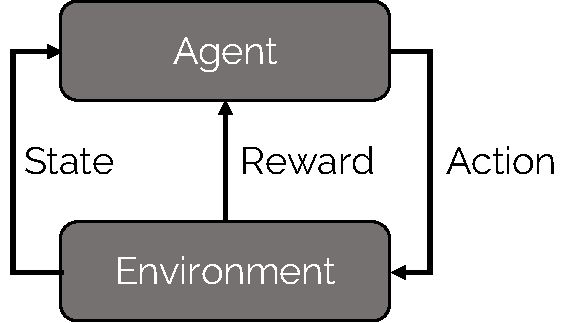
\includegraphics[width=0.3\textwidth]{RL_Fundamentals.pdf}
\caption{General concept of \acrfull{RL} as the interactions between the agent and its environment. The agent takes some action that has an impact on the environment which feeds back the agent with a reward and the new state. The objective of the agent is to optimize its policy, \ie mapping between the state it is at and the action to take, by maximizing its cumulative reward.}
\label{fig:RL_Fundamentals}
\end{figure}

The agent learns to optimize its policy by maximizing a notion of cumulative reward over time. This policy refers to the strategy or mapping from states to actions that the agent employs to make decisions. Essentially, it defines the behavior of the agent in the environment. The ultimate goal of the agent is often to find an optimal policy, which maximizes the expected cumulative reward over time.  All these concepts and interactions between the agent and its environment are formalized as a \gls{MDP} \cite{sutton2018reinforcement}, represented by the tuple $<s,a,T,r,\pi,\gamma>$.  The Markov property of such a decision process states that a decision is made only based on this tuple and not on the history/path that has led to it. In this tuple, $s\in S$ is the state defined in a certain state space, $S$, that represents the observable parts of the environment that the agent uses to make decisions; $a\in A$ is the action among the action space, $A$; $T$ is the probability of transitioning from one state $s$ to another state $s'$ given a specific action, $a$: $T(s,a,s'): \text{Pr}\left(s'|s,a\right)$; $r$ is the reward received by the agent when taking the action $a$ from state $s$, $R(s,a)$; $\pi$ is the policy telling the action to take depending on the current state and; $\gamma$ is the discount factor that controls the importance of future rewards versus immediate rewards. During the learning/optimization process, the agent acts according to the exploitation-exploration trade-off. In the exploitation, the action $a$ is directly given by the mapping provided by the current policy $\pi$,  depending on the state $s$. In the exploration, the action is randomly picked within the action space. For further information, the interested reader is invited to refer to work of \citet{sutton2018reinforcement} or the course given by \citet{davidsilver_RL_online} available online.

Due to the increasing complexity of the systems and the integration of uncertainties, the last decades have seen the emergence of publications where \gls{RL} is applied to energy systems \cite{cao2020reinforcement,perera2021applications}. In their respective reviews, \citet{cao2020reinforcement} and \citet{perera2021applications} highlighted groups of problems addressed with \gls{RL} in the research field of energy systems: building energy management system (BEMS), optimization of dispatch and operational control closely linked with the energy market and the optimal power flow problem in the grid, micro-grid management, electro-mobility or even demand-side management or optimal control of energy system devices like maximum power point tracking (MPPT) of wind turbines and \gls{PV} panels.  The major novelty of this thesis is the application of \gls{RL} to a new kind of energy system problem: the optimization of the transition pathway of a whole-energy system. In this sense, the objective is to optimize and provide a policy to support this transition subject to uncertainties.

\subsection{Problem formulation and algorithm}
\label{subsec:meth_RL_algo}
At the initial state, \ie the energy system in 2020, the agent gets an initial observation, $\bm{o}_0$. An observation represents a set of the characteristics of the environment accessible to the agent for it to take the next action. The state, though, is the exhaustive list of these characteristics. Even though an observation is a subset of the state, this work uses these two words interchangeably. Then, it takes an action, $\bm{a}_0$, impacting its environment, \ie the energy system limited transition over the first decision window (2020-2030). Through this interaction with its environment, the agent is given a reward, $r_1=r\left(\bm{a}_0 | \bm{o}_0 \right)$, and ends up in a new state, \ie the energy system in 2025, characterised by a new observation, $\bm{o}_1$, and so on (see Figure \ref{fig:Schematics_RL}).


\begin{figure}[!htbp]
\centering
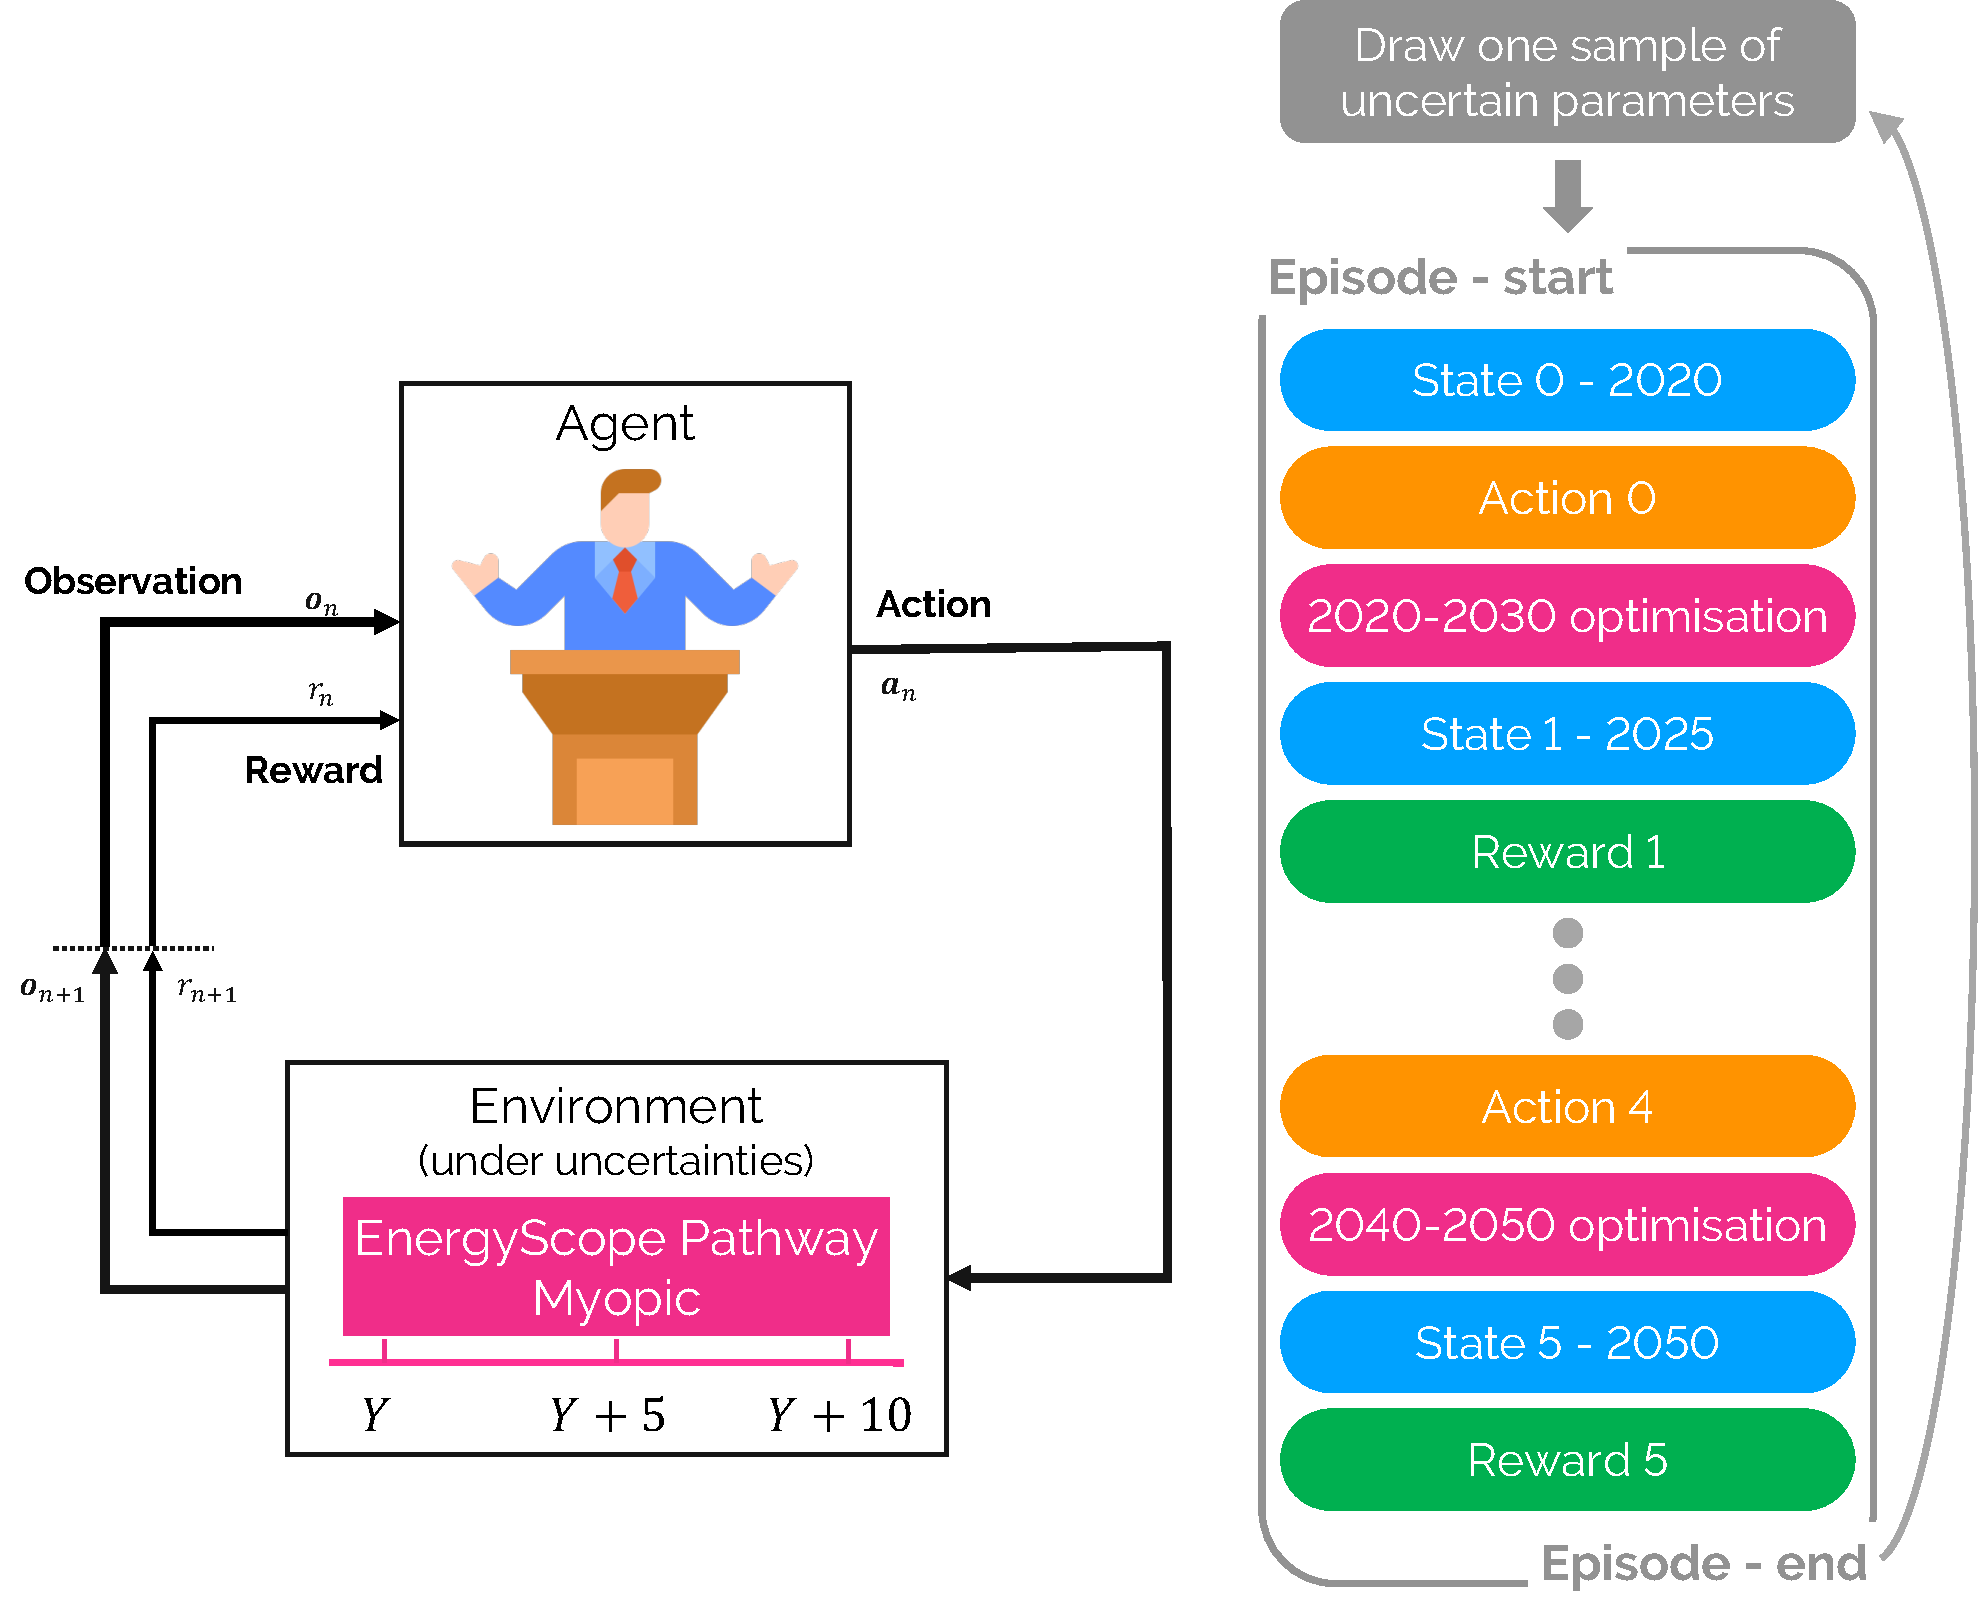
\includegraphics[width=0.8\textwidth]{Schematics_RL.pdf}
\caption{\Acrfull{RL} framework made of the agent interacting with its environment, \ie the energy-system model on a limited decision window of 10 years.}
\label{fig:Schematics_RL}
\end{figure}

A learning episode is a succession of such learning steps. In the context of the transition pathway between 2020 and 2050, an episode can come to an end for different reasons. First, if the actions taken by the agent make the optimisation infeasible, the episode is prematurely stopped before reaching 2050. Similarly, cumulative emissions of the system over the predefined \ce{CO2}-budget (see Section \ref{sec:cs:CO2-budget}) lead to an anticipated end of the episode. Finally, the ``natural'' end is the prescribed end of the transition, \ie 2050. Consequently, the maximum value of steps for an episode is equal to $N_{ep,max}=5$. 

Before jumping to the choice of the learning algorithm, it is worth noting that we opted for the combination of \gls{RL} with \gls{DNN}, called \gls{DRL}. Among others, one of the main drawbacks of traditional \gls{RL} algorithms, \ie without the use of \gls{NN},  is that it suffers from the ``curse of dimensionality'' when facing problems with continuous action and state spaces (see Chapter \ref{chap:chap_RL}). By approximating the state-action function with its parameters (\ie weights and biases), \gls{DNN} can address this difficulty. 

Given the assumed absence of knowledge of the agent about the dynamics of the environment, \ie its transition or reward functions, we needed a so-called ``model-free'' learning algorithm. In practice, in a model-free approach, the agent estimates the optimal policy directly from experience and without estimating the dynamics of the environment. However, model-free methods suffer from two major drawbacks: their sample inefficiency and their sensitivity with respect to their hyper-parameters (\eg learning rates, exploration constants) \cite{haarnoja2018soft}. The former leads to a too expensive computational burden while the second requires meticulous settings to get good results.  To overcome these two challenges, we needed to chose between an ``on-policy'' or ``off-policy'' algorithm. In a nutshell, in on-policy learning, the agent learns the value function or policy based on the data it generates by following its current policy whereas, in off-policy, the agent can learn from data collected by any policy, not just the one it is currently following, which provides greater flexibility and potential for reusing data. This makes off-policy algorithms more data efficient and ensuring better exploration by reusing past experiences or even following random exploration \cite{haarnoja2018soft}.

The goal of a \gls{RL} approach is to optimise the mapping between inputs (\ie the observations) and output (\ie the actions), called the policy $\pi\left(\bm{a}_n | \bm{o}_n\right)$. To do so, an objective function, $\bm{J}(\pi)$, is built on the cumulative rewards collected during each episode. Finally, a back-propagation process updates the weights and biases of the \gls{NN} during the learning of the agent. Among the wide variety of \gls{RL} algorithms applied in energy systems \cite{perera2021applications}, this work opted for \gls{SAC} \cite{haarnoja2018soft} to train and update the \gls{NN}.  Like other actor-critic-based algorithms, \gls{SAC} works with two \gls{NN} in parallel: the actor learning the control policy and the critic judging the actor (see Figure \ref{fig:Actor-critic}).

\begin{figure}[!htbp]
\centering
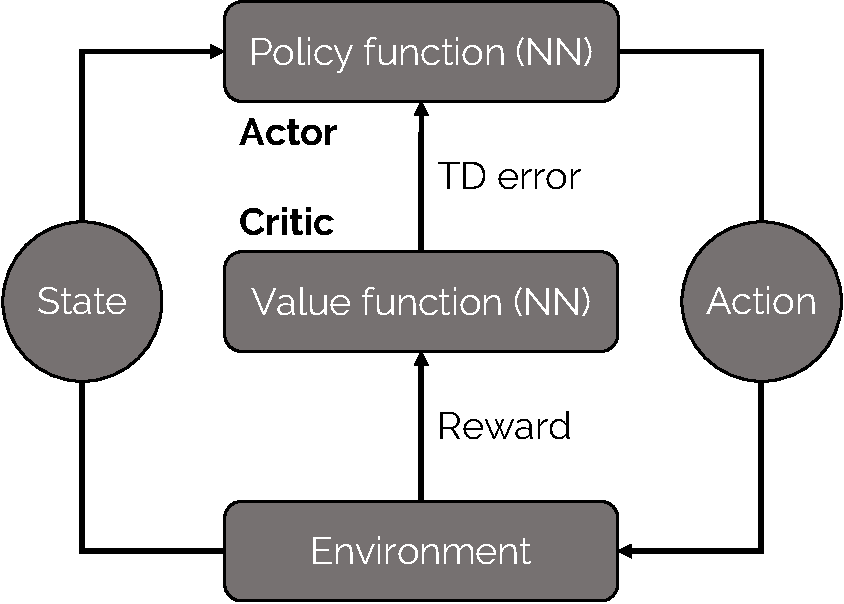
\includegraphics[width=0.5\textwidth]{Actor-critic.pdf}
\caption{General concept of actor-critic-based algorithms. The two \gls{NN} are trained against each other for the actor to improve the control policy and for the critic to provide a better judgement of the actor's action via the temporal-difference (TD) error. Graph adapted from \cite{cao2020reinforcement}.}
\label{fig:Actor-critic}
\end{figure}

\gls{SAC} is a model-free and off-policy actor-critic deep \gls{RL} algorithm based on the entropy-augmented\footnote{The word ``augmented'' here is in opposition to the conventional \gls{RL} objective function that is only based on the cumulative reward, \ie first term of Eq. \ref{eq:SAC_objective}.} objective function (see Eq. \ref{eq:SAC_objective}). Where entropy represents the amount of energy in a system not available to produce work in thermodynamics, this term, also called Shannon entropy in the \gls{RL} context, stands for the randomness or stochasticity of the policy.

\begin{equation}
    \label{eq:SAC_objective}
    \bm{J}(\pi) = \underset{\pi}{\mathbb{E}}\left[\underset{n=0}{\overset{N_{ep}}{\sum}}\gamma^n r_n\left(\bm{o}_n,\bm{a}_n \right) - \zeta \log \left(\pi\left(\bm{a}_n | \bm{o}_n\right) \right) \right],
\end{equation}

\noindent
where $\gamma$ is the discount factor and $\zeta$ the temperature parameter. $\gamma$ determines how much importance we want to give to future rewards within an episode. $\zeta$ balances the trade-off between exploitation of proven actions via the return maximisation, \ie $\sum_{n=0}^{N_{ep}}\gamma^n r_n\left(\bm{o}_n,\bm{a}_n \right)$, and exploration through the entropy term, \ie $\log \left(\pi\left(\bm{a}_n | \bm{o}_n\right) \right)$. This way, \gls{SAC} ensures sample efficiency while improving exploration \cite{haarnoja2017reinforcement} and robustness \cite{ziebart2010modeling}. In their work, \citet{haarnoja2017reinforcement} showed a lower sensitivity of \gls{SAC} to hyper-parameters. These make \gls{SAC} a state-of-the-art algorithm and one of the most efficient model-free deep RL method nowadays \cite{haarnoja2017reinforcement}. In this thesis, we used the open-source \gls{SAC} package developed by \textsc{Stable-Baselines3} \cite{raffin2021stable} where the policy \gls{NN} is a fully connected multilayer perceptron (MLP) built with \textsc{TensorFlow} \cite{abadi2016tensorflow}. For further information on \gls{RL} and the \gls{SAC} algorithm, the interested reader is invited to refer to the works of \citet{sutton2018reinforcement} and \citet{haarnoja2018soft}, respectively.

\section{Robustness assessment via PCA}
\label{sec:meth:PCA}
When optimizing a transition pathway of a whole-energy system, including its uncertainties, capturing the most variable changes of design (\ie installed capacities of each technology) can become overwhelming due to the curse of dimensionality. For the case study detailed in Chapter \ref{chap:case_study}, this consists of \ie 7 representative years of the transition (\ie from 2020 to 2050), 113 possible technologies subject to uncertain parameters. To tackle this challenge, we have developed a methodology based on the \acrfull{PCA}. The philosophy behind this approach is to identify key-combinations of design variables giving relevant dimensions to compare different systems, beyond their sole objective function, \ie total transition cost, but without having to compare each design variable individually. This methodology provides two main outputs. First and foremost, using the model runs necessary to quantify the impact of the uncertain parameters on the total cost of the transition (see Section \ref{sec:meth:UQ}), it gives a metric on which to assess the robustness of energy transition policies resulting from different approaches. This metric gives more insight that, for instance, the variation of the total transition cost that encompasses too many aspects (\ie design and operation strategies, variation along the transition) in one single value. Second, these ``directions of variation'' can highlight key modal shifts or highly varying design strategies over the transition. After introducing the general concept of \gls{PCA}, this section aims at detailing the methodology proposed to give these ``directions of variation'' and to assess the robustness of policies.

\subsection{Principal Component Analysis: General concept}
\label{subsec:meth:PCA:PCA}
Born in the early 20th century \cite{pearson1901on,hotelling1933analysis}, the \acrfull{PCA} finds its fundamentals from the \gls{SVD}. \gls{SVD} is a generalization, to an arbitrary (\ie not especially square) matrix, of the spectral theorem stating that a normal matrix can be diagonalized by an orthonormal basis of eigenvectors.  The core concept of principal component analysis (PCA) involves simplifying a dataset with numerous interconnected variables by reducing its dimensionality. The aim is to preserve as much variability within the data as feasible. This is accomplished by transforming the $p$-dimension data, $\mathbf{x}$, into a new set of variables called principal components (PCs), $\mathbf{z}$. These components are uncorrelated and arranged in such a way that the first ones retain the majority of the variability found in all of the original variables. On the other hand, the final principal components (PCs) pinpoint directions where there is minimal variation, indicating nearly constant linear relationships among the original variables \cite{jolliffe2002principal}. 

The PCs are computed based on the covariance matrix of $\mathbf{x}$, $\mathbf{\Sigma}$ where the diagonal of this matrix gives the variance of the $i^{\text{th}}$ variable and the other elements give the covariance between the $i^{\text{th}}$ and the $j^{\text{th}}$ variables where $i\neq j$. Out of this matrix, $\mathbf{\alpha_k}$ is the eigenvector of $\mathbf{\Sigma}$ corresponding to its $k^{\text{th}}$ highest eigenvalue $\lambda_k$. One crucial aspect of these eigenvectors is their normalization, \ie $\mathbf{\alpha_k}^{T}\mathbf{\alpha_k}=1$ \cite{jolliffe2002principal}. This normalization has several objectives. Among them, this ensures orthogonality of the PCs ensuring that they represent independent directions in the original feature space. Then, normalizing the eigenvectors ensures that the magnitude of each eigenvector represents the importance or variance explained by its corresponding principal component. This makes it easier to interpret the relative importance of each principal component in explaining the variability of the data. Finally, this ensures a fair comparison between the original features. Without normalization, variables with larger scales would dominate the principal components, potentially skewing the results and leading to misinterpretation of the principal components. In other words, given this normalization, $\mathrm{var}\left(z_k\right)=\lambda_k$, where $\mathrm{var}\left(z_k\right)$ is the variance of $z_k$. Moreover, this means that $\alpha_{ki}$, \ie the component of $ \mathbf{\alpha_k}$ related to the $i^{\text{th}}$ original variable, $x_i$,  gives its weight in the $k^{\text{th}}$ PC, \ie $z_k$. This PC captures $\lambda_k$ variance of the original data. In other words, a high absolute value of $\alpha_{ki}$ means that $x_i$ has a significant impact in the direction given by the $k^{\text{th}}$ PC \cite{zdybal2022advancing}. 

Easier to represent in two dimensions, let us consider a vector $\mathbf{x}$ composed of the variables $x_1$ and $x_2$, $p=2$, and 25 realisations of them (See Figure \ref{fig:PCA_intro} (left)). These realisations of the original variables allow building the covariance matrix. Then, the first \gls{PC}, $z_1$, is a linear function, $\mathbf{\alpha_1^{T}x}$,  of the different variables of $\mathbf{x}$ with maximum variance:

\begingroup
\belowdisplayskip=2pt
\abovedisplayskip=2pt
\begin{flalign}
\hspace{0pt}
  \label{eq:PCA_z1}%7
 z_1=\sum_{j=1}^{p} \alpha_{1j}x_j=\mathbf{\alpha_1^{T}x}=\alpha_{11}x_1+\alpha_{12}x_2,
\end{flalign}
\endgroup

\noindent
where $\mathbf{^T}$ means the transpose vector. Then, $z_2=\mathbf{\alpha_2^{T}x}$, is another linear function of $\mathbf{x}$,uncorrelated with $z_1$ and maximizing the variance. These linear transformations can be seen as projection of the original data on the principal direction, \ie PCs (see Figure \ref{fig:PCA_intro} (right)). In more general cases, one can write $z_k=\mathbf{\alpha_k^{T}x}$ as the $k^{\text{th}}$ PC. There can be up to $p$ PCs even though, usually, most of the variance of the original data can be captured by $m$ PCs where $m\ll p$. The interested reader is invited to refer to the work of \citet{jolliffe2002principal} for further mathematical demonstrations, information and examples.

\begin{figure}[!htbp]
\centering
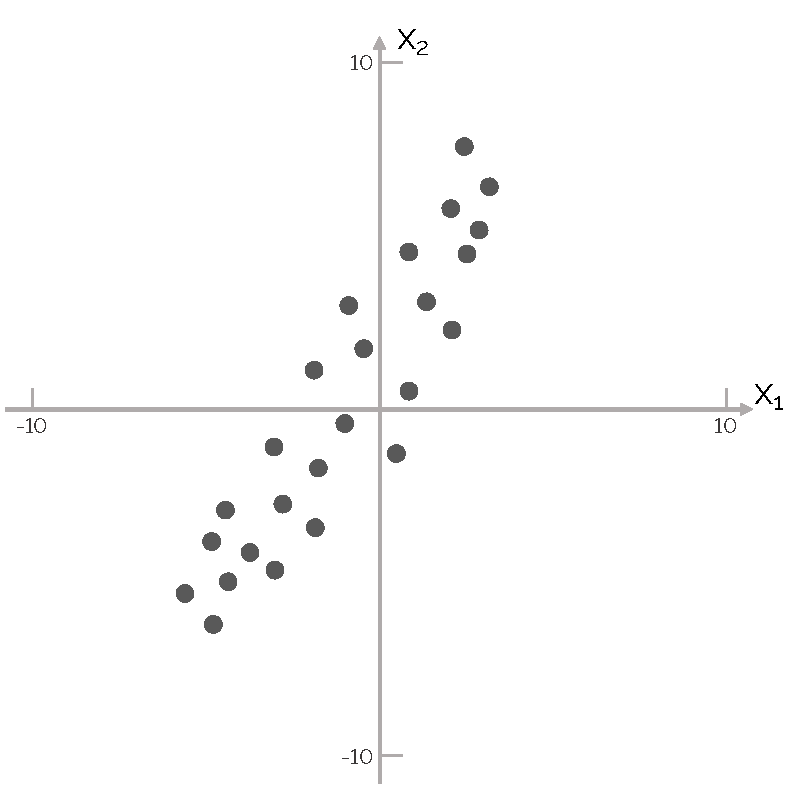
\includegraphics[width=0.4\textwidth]{PCA_intro_original.pdf}
\hspace{1.5cm}
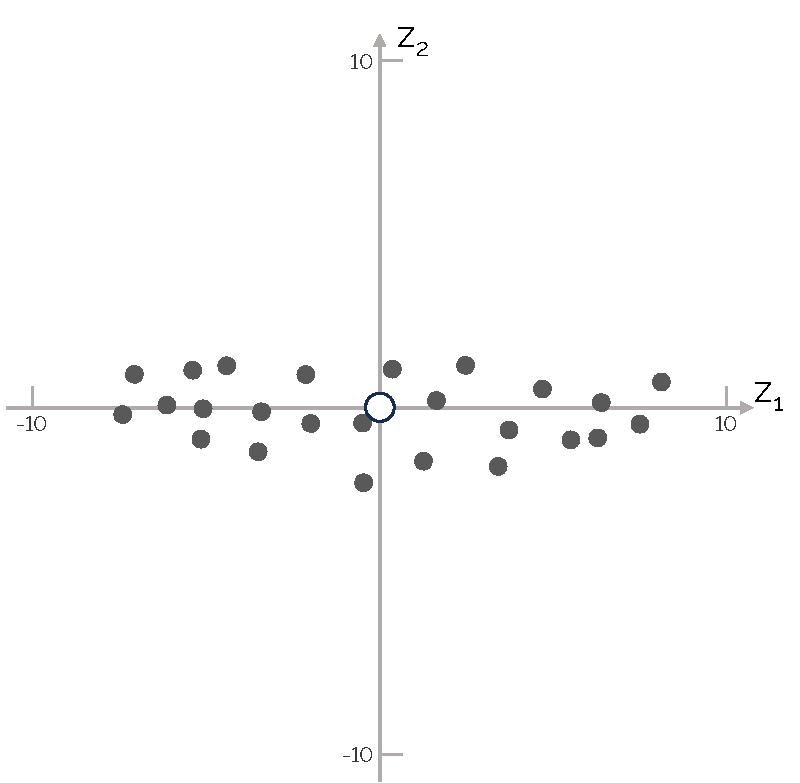
\includegraphics[width=0.4\textwidth]{PCA_intro_PCA.pdf}
\caption{Original observations of the dataset (left) and their projection with respect to their PCs (right). The variation of the realisations is more significant in the direction of $x_2$ than $x_1$. Once projected with respect to their PCs, the variation is even more significant in the direction of $z_1$ than in either of the original variables, as it captures most of their variance. Graph adapted from \cite{jolliffe2002principal}.}
\label{fig:PCA_intro}
\end{figure}

\subsection{Principal components of the transition}
\label{subsec:meth:PCA:transition}
As introduced, the objective is to define the main technological drivers of the variation through the transition to 2050 subject to uncertainties. To do so, before calculating the PCs of the transition, three preliminary steps are necessary: (i) selection of the right data, (ii) data scaling and, (iii) outliers management. Like any other dimension-reduction process, \gls{PCA} has to be supplied with relevant data to reach the stated objective.  Like the normalization of the eigenvectors (see Section \ref{subsec:meth:PCA:PCA}), data scaling is fundamental to compare features having potentially different units and/or order of magnitude. Finally, properly handling the outliers allows reaching the relevant level of metric between the too vague information of the sole total transition cost and too many details hidden in the peculiar/outlying cases. After this preprocessing, PCs can be computed for each of the year of the transition then aggregated to give a bigger picture over the whole transition.\\

\myparagraph{Data selection}\\

\noindent
To characterize the variations of design within the transition under uncertainties, we have focused on the installed capacities, $\textbf{F}(y,j)$ for all $y \in \text{\emph{YEARS}}$ and $j \in \text{\emph{TECH}}$ (see Eq. \ref{eq:F_newBuilt}). Even though these represent only the design part of the result of the optimization, along with the operation, focusing on the installed capacities give a direct information regarding the required capital investment (see Eq. \ref{eq:c_inv}) and, more indirectly, the resources to use.  In other words, it captures the technological landscape of the transition.  Having defined the type of variable to consider, we need to assemble a relevant dataset. This is given by the runs to quantify the impact of the uncertain parameters on the total cost of transition required by the method described in Section \ref{sec:meth:UQ}. Overall, the original dataset is $\textbf{x}(y,j,s)$ where, on top of $y$ and $j$ previously defined, $s \in [1,2,...,S]$ stands for the sample number of the uncertainty quantification method. For the investigated case detailed in Chapter \ref{chap:atom_mol}, this represents $S=240$ samples resulting from the perfect foresight optimization of the transition pathway under uncertainties. Finally, among the seven representative years of the transition, we do not consider 2020 as it is the initialisation year for which the design of the system is fixed, to be representative of the actual design that was in place (see Appendix \ref{app:bel_2020}). In other words, we focus here only on the years 2025, 2030, 2035, 2040, 2045 and 2050. This gives the whole dataset considered in this \gls{PCA} (see Figure \ref{fig:PCA_data}).\\

\begin{figure}[!htbp]
\centering
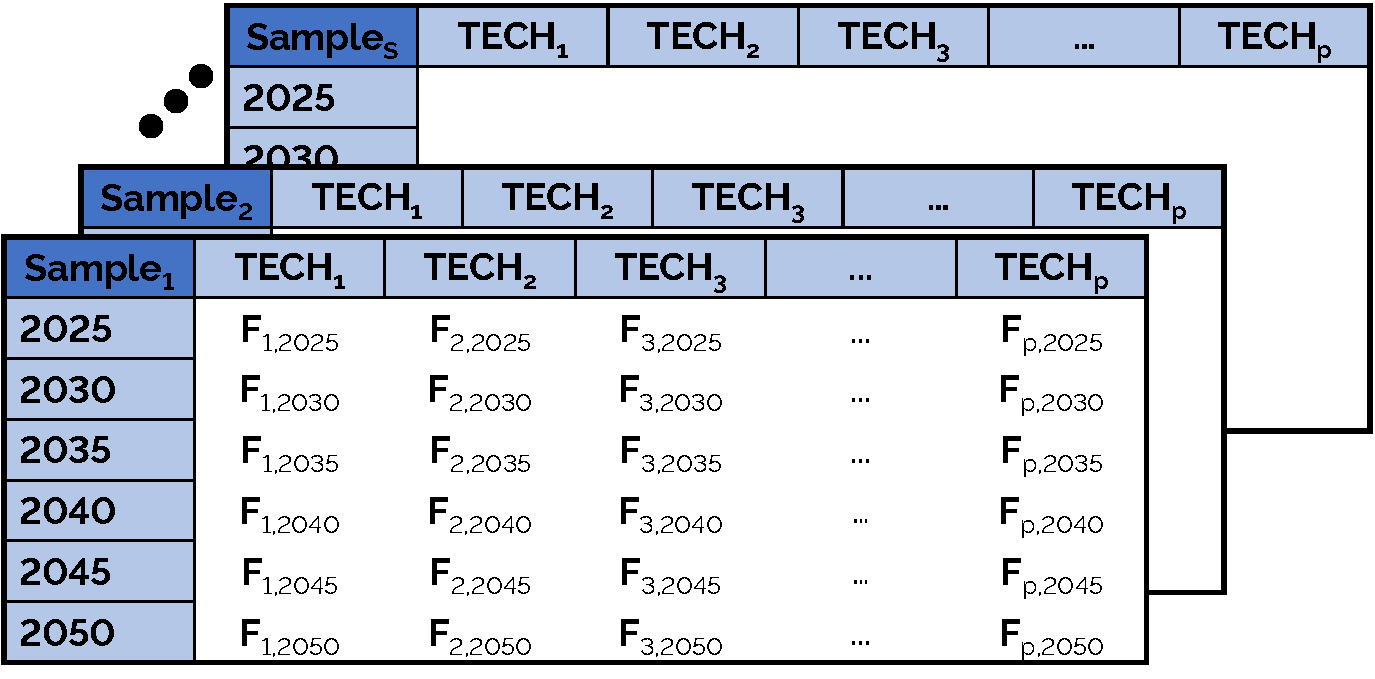
\includegraphics[width=0.8\textwidth]{PCA_data.pdf}
\caption{Original raw data considered in the \acrfull{PCA} of the variation of the design strategy through the transition, $\textbf{x}(y,j,s)$, accounting for the $p$ possible technologies to install.}
\label{fig:PCA_data}
\end{figure}

\myparagraph{Data scaling}\\

\noindent
Preprocessing the dataset before employing a method to reduce dimensionality, like \gls{PCA}, can greatly affect the structure of the simplified representation and the characteristics of the features extracted from the dataset \cite{parente2013principal,peerenboom2015dimension}. Scaling the original raw data via normalization, \ie reducing data to $[0, 1]$ interval has a double purposes: to assess variables (i) representing different sorts of features, with different units (\eg installed capacity of electricity and mobility technologies) and, (ii) ranging over the different orders of magnitude (\eg installed capacity of private and public mobility) (see Appendix \ref{app:bel_2020}).  Consequently, the first part of this data preprocessing consists in scaling the installed capacities versus their respective sector and representative year (see Eq. \ref{eq:PCA_scaling_0}). The sectors, as defined in EnergyScope, are the electricity, \gls{HT} heat, \gls{LT} heat, passenger mobility, freight mobility, \gls{NED}, storage and infrastructures. For instance, the installed capacity of \gls{PV} panels in the year $y$ of the sample $s$ is scaled by the maximum installed capacity in the electricity sector in the year $y$ among all the samples.

\begin{equation}
 \label{eq:PCA_scaling_0}
\textbf{x}^{*}(y,j,s)=\frac{\textbf{x}(y,j,s)}{\mathrm{max}_{sec,y}\left(\textbf{x}(y,j,s)\right)}
 \quad \forall y \in \text{\emph{YEARS}}, sec \in \text{\emph{SECTORS}}
\end{equation}

Then, to give ``directions/metrics'' representative to the size of each sector within the energy system, we added another weight based on the relative share of commodity produced by each sector. For the case study of Belgium detailed in Chapter \ref{chap:case_study}, this gives a higher weight for electricity and low-temperature heat sectors (see Figure \ref{fig:Share_EUD_sectors}). 

\begin{figure}[!htbp]
\centering
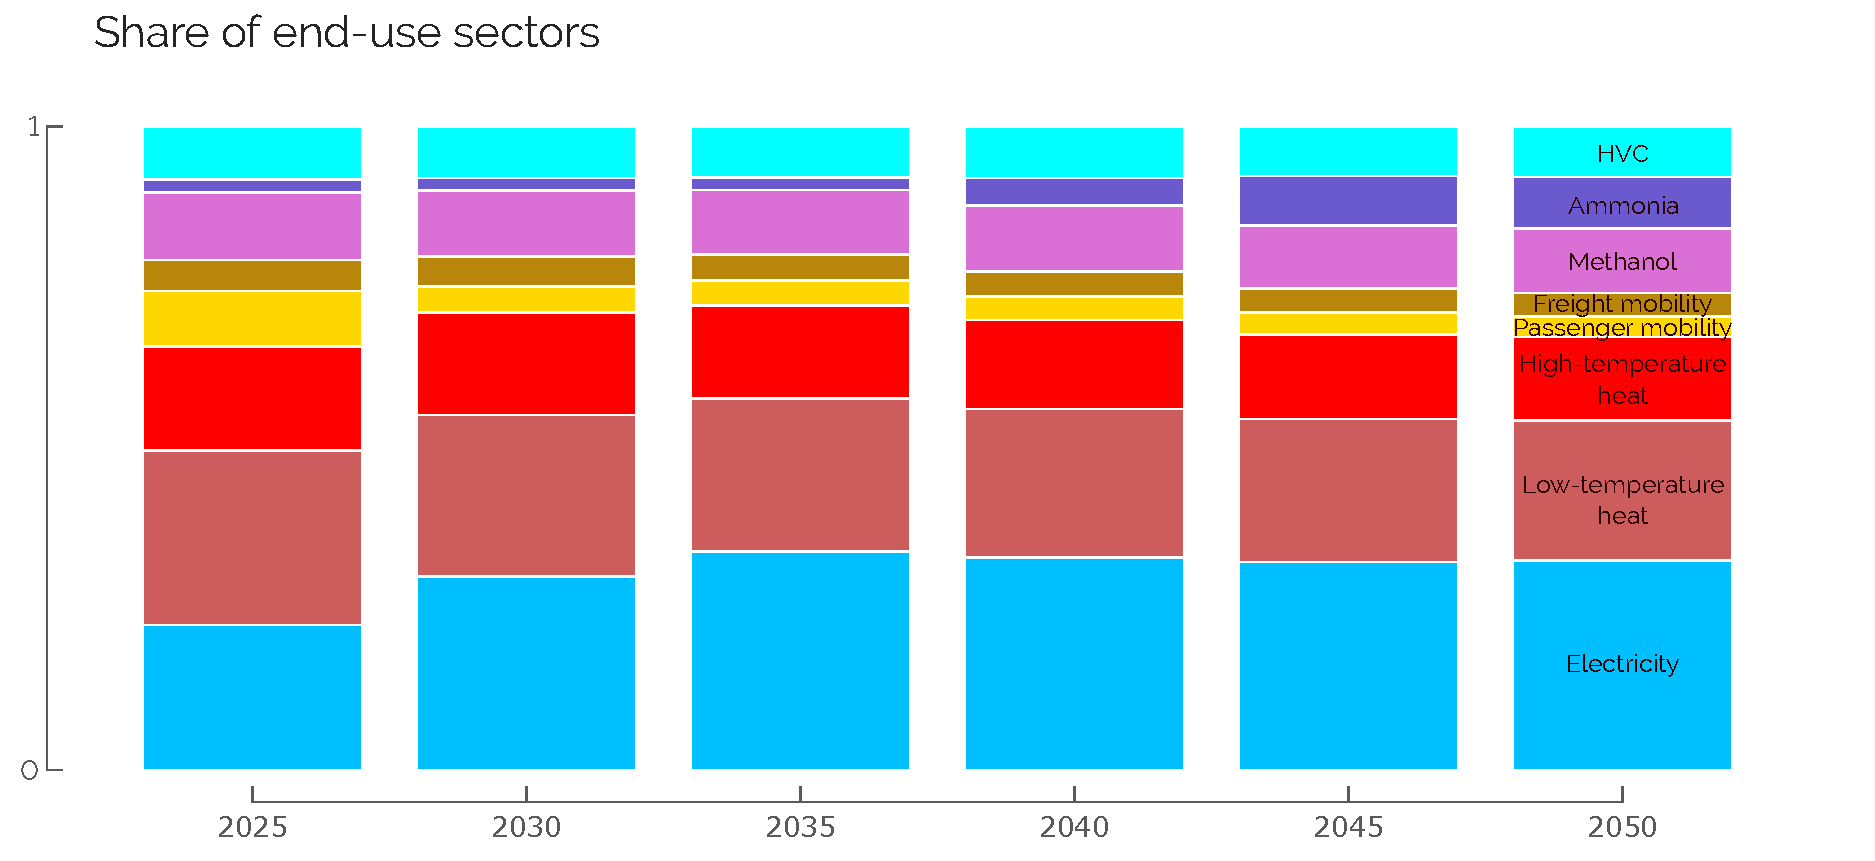
\includegraphics[width=0.8\textwidth]{Share_EUD_sectors.pdf}
\caption{Multiplying factor for each of the end-use sectors in the case of Belgian energy transition. These shares are based on results of the reference scenario (REF) where nominal values are considered for the uncertain parameters and the transition is optimized through the perfect foresight approach. Over the transition, sectors like electricity (\ie from 22\% in 2025 to 33\% in 2050) or ammonia (\ie from 2\% to 8\%) become more important due to sector coupling, \eg e-mobility or ammonia-\gls{CCGT}.}
\label{fig:Share_EUD_sectors}
\end{figure}

To do so, we have arbitrarily considered these shares from the REF case, where the pathway is optimized according to the perfect foresight approach and considering all the uncertain parameters to their nominal value (see Chapter \ref{chap:atom_mol}).  The end-use-demands as well as the commodity produced for the sector coupling are based on the results of this deterministic REF case.  For instance, the share of the electricity sector accounts for its \gls{EUD} and the electricity produced to supply other sectors (\eg heat, mobility). Finally, to compare apples with apples, we converted the \gls{EUD} in the mobility sectors, \ie passenger and freight, into the \gls{FEC} they require in the REF case. This gives the second weighing factor to scale data, on top of the one of Eq. \ref{eq:PCA_scaling_0} (see Eq. \ref{eq:PCA_scaling_1}).

\begin{equation}
 \label{eq:PCA_scaling_1}
\textbf{x}^{**}(y,j,s)=\textbf{x}^{*}(y,j,s)\cdot \text{share}_{\text{EUD}}(y,sec)
 \quad \forall y \in \text{\emph{YEARS}}, sec \in \text{\emph{SECTORS}}
\end{equation}

One would notice that this second scaling factor omits the infrastructure and storage technologies. In the process to define ``metrics'' to assess the robustness of a policy for the case of Belgium, this has a negligible impact. Indeed, the variation of the installed capacity of these technologies are either limited compared to end-use-type (EUT) technologies, \ie limiting their influence in the definition of PCs, or directly linked to these EUT technologies (\eg \gls{DHN} installed capacity is directly proportional to technologies producing \gls{LT} heat in \gls{DHN} or the additional capacity of grid is caused by additional capacities of \gls{VRES}). \\

\myparagraph{Outliers management}\\

\begin{wrapfigure}{r}{3cm}
\centering
\captionsetup{justification=centering}
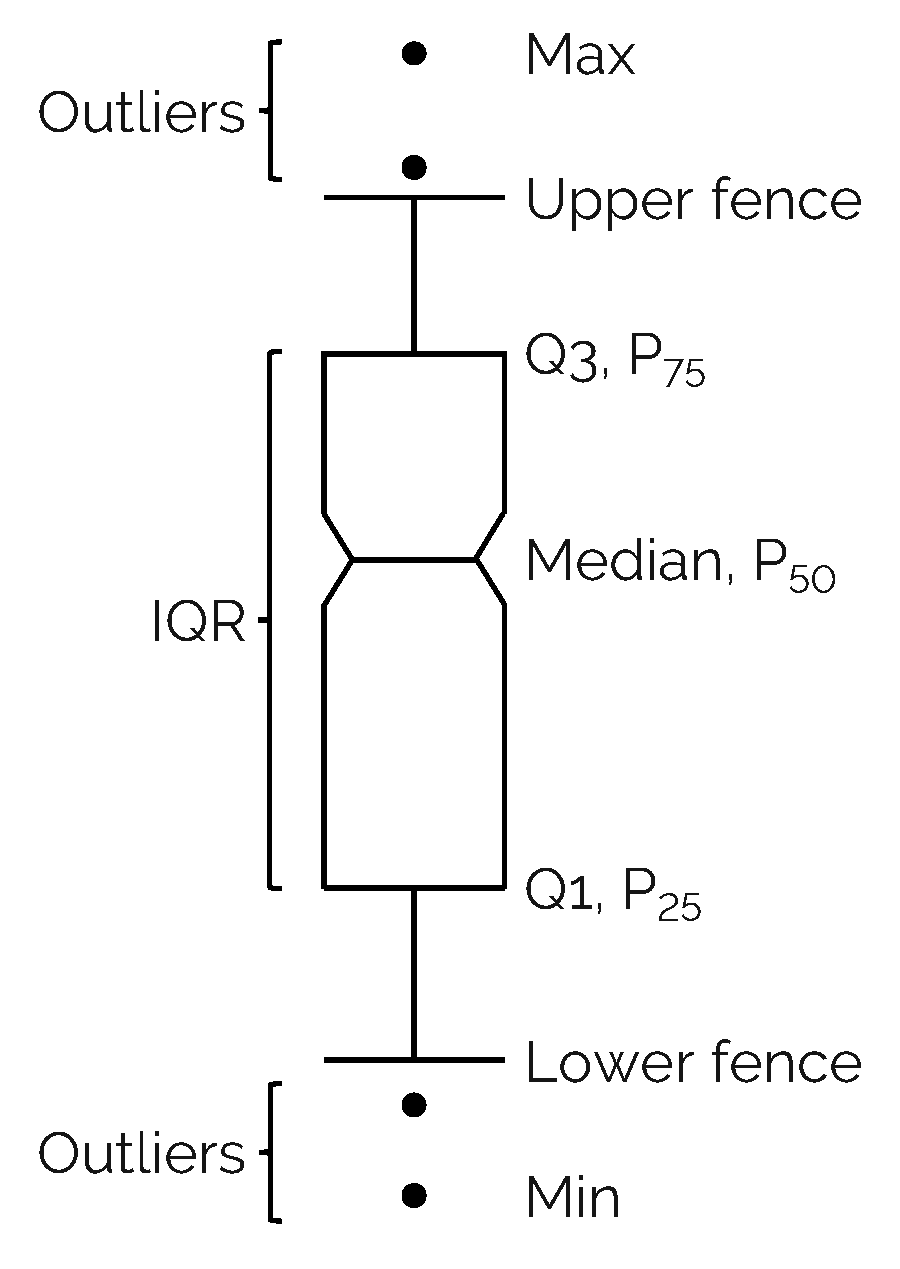
\includegraphics[width=2.8cm]{Schematic_boxplot.pdf}
\caption{}
\label{fig:Schematic_boxplot_methodo}
\end{wrapfigure}

\noindent
Handling outliers is one of the biggest challenges in data science \cite{aguinis2013best}. These are defined as data points differing significantly from the rest of the data set. Being extreme values, outliers influence the overall dataset variance and, consequently, rotate the PCs directions towards them \cite{stanimirova2007dealing}. In the context of \gls{PCA}, outliers could be defined as ``model fit outliers'' as their presence influences the fit of the model. There are several techniques to detect/define and handle the outliers \cite{aguinis2013best}. In this work, detection is performed via the box plot technique, as outliers are identified as those points lying beyond the plot’s whiskers, or fences. These whiskers are themselves constructed as being 1.5 times the \gls{IQR} (Q3 - Q1) higher or lower than the third (Q3) or first quartile (Q1), respectively (see Figure \ref{fig:Schematic_boxplot_methodo}). Therefore, the installed capacity of a technology in the year $y$ of the sample $s$ is defined as an outlier if it falls out of this range compared to the rest of the dataset for this specific technology and year across all the samples. There exist several techniques to handle these outliers depending on their nature or the method used to identify them. Since all the data points correspond to a result provided by the optimization, we have decided to keep these points but carry out a modification of them \cite{aguinis2013best}. In practice,  the value of ``high outliers'' or ``low outliers'' is set to the upper or lower fence, respectively. In practice, this modification narrows the variation range of features presenting outliers and, consequently, reduces their weight in the different PCs.\\

\myparagraph{Principal components of each representative year}\\

\noindent
Now that data are selected and preprocessed, principal components are first computed for each representative year separately, using the Python package \textsc{PCA} from \textsc{sklearn.decomposition}. As explained in Section \ref{subsec:meth:PCA:PCA}, the number of PCs per year to retain can go up to the number of considered variables (\ie 73\footnote{73 technologies out of the 113 in total as we do not consider the 15 infrastructure technologies nor the 25 storage technologies.} in our case study) which is intractable. Moreover, the first PCs keep track of most of the variance of the system whereas the last ones present a smaller interest. Choosing the appropriate threshold involves a trade-off. Retaining too few principal components may result in loss of important information, while retaining too many may lead to unclear analysis. In this work is to compute, for each of the representative years of the transition (except 2020),  the PCs capture 90\% of the total variance of this year \cite{jolliffe2002principal}. At the end of this step, we have a list of $m$ PCs, \ie $\text{PC}_{y,i}$ where $y$ stands for the year between 2025 and 2050 and 

\begin{equation}
\label{eq:PC_year}
\sum_{i=0}^m\text{var}\left(\text{PC}_{y,i}\right)\geq 90\% \sum_{i=0}^p\text{var}\left(\text{PC}_{y,i}\right) \quad \forall y \in \text{\emph{YEARS}},
\end{equation}

\noindent
where $m$ is presumably different for each representative year and $p$ is the total number of variables, hence the maximum number of PCs. For the entire transition, it gives a total of $M$ $\text{PC}_{y,i}$.\\

\myparagraph{Principal components of the transition}\\

\noindent
The final step consists in defining metrics on the whole transition based on the $\text{PC}_{y,i}$ computed for each representative year, separately. To do so, all the $\text{PC}_{y,i}$ from every year are sorted together in a descending order based on their respective variance. Then, starting with the one with the highest absolute variance, all the other $\text{PC}_{y,i}$ similar to it are clustered together. The similarity between two PCs is defined according to the cosine similarity approach, especially appropriate in high-dimensional positive spaces \cite{xia2015learning}. Indeed, as detailed in Section \ref{subsec:meth:PCA:PCA}, a PC represents a vector for which the components are related to each variable of interest. Therefore, in this work, PCs are considered similar if their cosine similarity, $S_C (A,B)$, is greater or equal to 90\%:

\begin{equation}
\label{eq:cos_similarity}
S_C (A,B):= \cos(\theta) = {\mathbf{A} \cdot \mathbf{B} \over \|\mathbf{A}\| \|\mathbf{B}\|} = \frac{ \sum\limits_{i=1}^{n}{A_i  B_i} }{ \sqrt{\sum\limits_{i=1}^{n}{A_i^2}} \cdot \sqrt{\sum\limits_{i=1}^{n}{B_i^2}} } \geq 90\%,
\end{equation}

\noindent
where $A$ and $B$ represent two different PCs.  The components of these similar PCs are then averaged to form the first PC of the transition, $\text{PC}_{\text{transition},1}$. Then, the process repeats with the $\text{PC}_{y,i}$ with the highest absolute variance but that has not been integrated in the construction of $\text{PC}_{\text{transition},1}$, to form $\text{PC}_{\text{transition},2}$. This goes on until the sum of the absolute variance of the $N$ $\text{PC}_{y,i}$ used to construct these $\text{PC}_{\text{transition}}$ is greater or equal to 90\% of the sum of the absolute variance of all the $M$ $\text{PC}_{y,i}$ generated at the previous step:

\begin{equation}
\label{eq:PC_transition}
\sum_{i=0}^N\text{var}\left(\text{PC}_{y,i}\right)\geq 90\% \sum_{i=0}^M\text{var}\left(\text{PC}_{y,i}\right)
\end{equation}


\myparagraph{Robustness assessment of roadmaps}\\

\noindent
Similarly to the work of \citet{moret2020overcapacity}, roadmaps are defined by setting minimal installed capacities based on the results of different transition pathway optimizations (see Chapter \ref{chap:chap_RobPol}). The $\text{PC}_{\text{transition}}$ are the ``direction/metrics'' on which are projected the results from the myopic pathway optimization subject to minimal installed capacities set by these roadmaps.  In conclusion, a roadmap would be defined as more robust than another one if the projection of its myopic runs on the different $\text{PC}_{\text{transition}}$ spans on a more narrow range (see Figure \ref{fig:Projection_PC_transition}). The bounds of this ``range of projection'' are computed as the mean, $\mu$, of the projected data $\pm$ a 95\% confidence level, CL, on the margin of error, MOE:
$$
\text{range of projection} = [\mu-\mathrm{MOE}; \mu + \mathrm{MOE}],
$$

\noindent
where the margin of error, MOE,  is computed thanks to standard error of the mean, SEM, and assuming a Student's, distribution, t,  of the $N$ projected data:
$$
\text{MOE} = \mathrm{SEM}\cdot \mathrm{PPF}_{\mathrm{t}}\left((1+\mathrm{CL})/2,N-1\right),
$$

\noindent
where $\mathrm{PPF}_{\mathrm{t}}$ is the percent point function (\ie inverse of cumulative distribution function) of the Student's distribution.

\begin{figure}[!htbp]
\centering
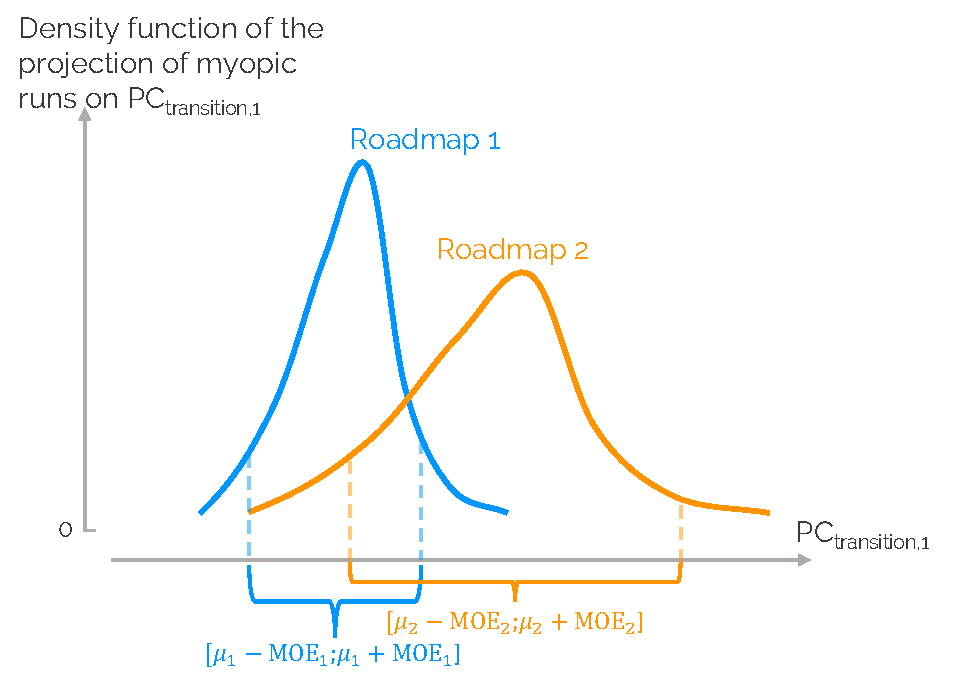
\includegraphics[width=0.8\textwidth]{Projection_PC_transition.pdf}
\caption{Projection on the first PC of the transition, $\text{PC}_{\text{transition},1}$, of the different myopic runs under uncertainties based on different roadmaps. Given that the distribution resulting from roadmap 1 spans over a more narrow range of this PC of the transition, we conclude that this roadmap is more robust than roadmap 2 according to the direction of variation described by $\text{PC}_{\text{transition},1}$.}
\label{fig:Projection_PC_transition}
\end{figure}

